\documentclass[]{article}
\usepackage{lmodern}
\usepackage{amssymb,amsmath}
\usepackage{ifxetex,ifluatex}
\usepackage{fixltx2e} % provides \textsubscript
\ifnum 0\ifxetex 1\fi\ifluatex 1\fi=0 % if pdftex
  \usepackage[T1]{fontenc}
  \usepackage[utf8]{inputenc}
\else % if luatex or xelatex
  \ifxetex
    \usepackage{mathspec}
  \else
    \usepackage{fontspec}
  \fi
  \defaultfontfeatures{Ligatures=TeX,Scale=MatchLowercase}
\fi
% use upquote if available, for straight quotes in verbatim environments
\IfFileExists{upquote.sty}{\usepackage{upquote}}{}
% use microtype if available
\IfFileExists{microtype.sty}{%
\usepackage{microtype}
\UseMicrotypeSet[protrusion]{basicmath} % disable protrusion for tt fonts
}{}
\usepackage[margin=1in]{geometry}
\usepackage{hyperref}
\hypersetup{unicode=true,
            pdftitle={MBD: The Multiple Birth-Death model},
            pdfauthor={Giovanni Laudanno},
            pdfborder={0 0 0},
            breaklinks=true}
\urlstyle{same}  % don't use monospace font for urls
\usepackage{color}
\usepackage{fancyvrb}
\newcommand{\VerbBar}{|}
\newcommand{\VERB}{\Verb[commandchars=\\\{\}]}
\DefineVerbatimEnvironment{Highlighting}{Verbatim}{commandchars=\\\{\}}
% Add ',fontsize=\small' for more characters per line
\usepackage{framed}
\definecolor{shadecolor}{RGB}{248,248,248}
\newenvironment{Shaded}{\begin{snugshade}}{\end{snugshade}}
\newcommand{\AlertTok}[1]{\textcolor[rgb]{0.94,0.16,0.16}{#1}}
\newcommand{\AnnotationTok}[1]{\textcolor[rgb]{0.56,0.35,0.01}{\textbf{\textit{#1}}}}
\newcommand{\AttributeTok}[1]{\textcolor[rgb]{0.77,0.63,0.00}{#1}}
\newcommand{\BaseNTok}[1]{\textcolor[rgb]{0.00,0.00,0.81}{#1}}
\newcommand{\BuiltInTok}[1]{#1}
\newcommand{\CharTok}[1]{\textcolor[rgb]{0.31,0.60,0.02}{#1}}
\newcommand{\CommentTok}[1]{\textcolor[rgb]{0.56,0.35,0.01}{\textit{#1}}}
\newcommand{\CommentVarTok}[1]{\textcolor[rgb]{0.56,0.35,0.01}{\textbf{\textit{#1}}}}
\newcommand{\ConstantTok}[1]{\textcolor[rgb]{0.00,0.00,0.00}{#1}}
\newcommand{\ControlFlowTok}[1]{\textcolor[rgb]{0.13,0.29,0.53}{\textbf{#1}}}
\newcommand{\DataTypeTok}[1]{\textcolor[rgb]{0.13,0.29,0.53}{#1}}
\newcommand{\DecValTok}[1]{\textcolor[rgb]{0.00,0.00,0.81}{#1}}
\newcommand{\DocumentationTok}[1]{\textcolor[rgb]{0.56,0.35,0.01}{\textbf{\textit{#1}}}}
\newcommand{\ErrorTok}[1]{\textcolor[rgb]{0.64,0.00,0.00}{\textbf{#1}}}
\newcommand{\ExtensionTok}[1]{#1}
\newcommand{\FloatTok}[1]{\textcolor[rgb]{0.00,0.00,0.81}{#1}}
\newcommand{\FunctionTok}[1]{\textcolor[rgb]{0.00,0.00,0.00}{#1}}
\newcommand{\ImportTok}[1]{#1}
\newcommand{\InformationTok}[1]{\textcolor[rgb]{0.56,0.35,0.01}{\textbf{\textit{#1}}}}
\newcommand{\KeywordTok}[1]{\textcolor[rgb]{0.13,0.29,0.53}{\textbf{#1}}}
\newcommand{\NormalTok}[1]{#1}
\newcommand{\OperatorTok}[1]{\textcolor[rgb]{0.81,0.36,0.00}{\textbf{#1}}}
\newcommand{\OtherTok}[1]{\textcolor[rgb]{0.56,0.35,0.01}{#1}}
\newcommand{\PreprocessorTok}[1]{\textcolor[rgb]{0.56,0.35,0.01}{\textit{#1}}}
\newcommand{\RegionMarkerTok}[1]{#1}
\newcommand{\SpecialCharTok}[1]{\textcolor[rgb]{0.00,0.00,0.00}{#1}}
\newcommand{\SpecialStringTok}[1]{\textcolor[rgb]{0.31,0.60,0.02}{#1}}
\newcommand{\StringTok}[1]{\textcolor[rgb]{0.31,0.60,0.02}{#1}}
\newcommand{\VariableTok}[1]{\textcolor[rgb]{0.00,0.00,0.00}{#1}}
\newcommand{\VerbatimStringTok}[1]{\textcolor[rgb]{0.31,0.60,0.02}{#1}}
\newcommand{\WarningTok}[1]{\textcolor[rgb]{0.56,0.35,0.01}{\textbf{\textit{#1}}}}
\usepackage{longtable,booktabs}
\usepackage{graphicx,grffile}
\makeatletter
\def\maxwidth{\ifdim\Gin@nat@width>\linewidth\linewidth\else\Gin@nat@width\fi}
\def\maxheight{\ifdim\Gin@nat@height>\textheight\textheight\else\Gin@nat@height\fi}
\makeatother
% Scale images if necessary, so that they will not overflow the page
% margins by default, and it is still possible to overwrite the defaults
% using explicit options in \includegraphics[width, height, ...]{}
\setkeys{Gin}{width=\maxwidth,height=\maxheight,keepaspectratio}
\IfFileExists{parskip.sty}{%
\usepackage{parskip}
}{% else
\setlength{\parindent}{0pt}
\setlength{\parskip}{6pt plus 2pt minus 1pt}
}
\setlength{\emergencystretch}{3em}  % prevent overfull lines
\providecommand{\tightlist}{%
  \setlength{\itemsep}{0pt}\setlength{\parskip}{0pt}}
\setcounter{secnumdepth}{5}
% Redefines (sub)paragraphs to behave more like sections
\ifx\paragraph\undefined\else
\let\oldparagraph\paragraph
\renewcommand{\paragraph}[1]{\oldparagraph{#1}\mbox{}}
\fi
\ifx\subparagraph\undefined\else
\let\oldsubparagraph\subparagraph
\renewcommand{\subparagraph}[1]{\oldsubparagraph{#1}\mbox{}}
\fi

%%% Use protect on footnotes to avoid problems with footnotes in titles
\let\rmarkdownfootnote\footnote%
\def\footnote{\protect\rmarkdownfootnote}

%%% Change title format to be more compact
\usepackage{titling}

% Create subtitle command for use in maketitle
\providecommand{\subtitle}[1]{
  \posttitle{
    \begin{center}\large#1\end{center}
    }
}

\setlength{\droptitle}{-2em}

  \title{MBD: The Multiple Birth-Death model}
    \pretitle{\vspace{\droptitle}\centering\huge}
  \posttitle{\par}
    \author{Giovanni Laudanno}
    \preauthor{\centering\large\emph}
  \postauthor{\par}
      \predate{\centering\large\emph}
  \postdate{\par}
    \date{2019-07-25}

\usepackage{bbm}

\begin{document}
\maketitle

{
\setcounter{tocdepth}{2}
\tableofcontents
}
Install the package:

\begin{Shaded}
\begin{Highlighting}[]
\ControlFlowTok{while}\NormalTok{ (}\OperatorTok{!}\KeywordTok{require}\NormalTok{(devtools)) \{}\KeywordTok{install.packages}\NormalTok{(}\StringTok{"devtools"}\NormalTok{)\};}
\CommentTok{#> Carico il pacchetto richiesto: devtools}
\NormalTok{devtools}\OperatorTok{::}\KeywordTok{install_github}\NormalTok{(}\StringTok{"Giappo/mbd@debug"}\NormalTok{);}
\CommentTok{#> Skipping install of 'mbd' from a github remote, the SHA1 (dd948aef) has not changed since last install.}
\CommentTok{#>   Use `force = TRUE` to force installation}
\KeywordTok{library}\NormalTok{(mbd);}
\end{Highlighting}
\end{Shaded}

\hypertarget{the-theory}{%
\section{The theory}\label{the-theory}}

\hypertarget{the-process}{%
\subsection{The process}\label{the-process}}

Mbd stands for Multiple-Birth-Death. It is a model that includes the possibility
of the occurrance of multiple simultaneous speciations at any given time.
The process allows 3 possible events to occurr:

\begin{itemize}
\tightlist
\item
  single speciation, with rate \(\lambda\);
\item
  extinction, with rate \(\mu\);
\item
  multiple speciation, with rate \(\nu\). Then, if it occurs, each of the species present has probability \(q\) to speciate;
\end{itemize}

Parameters \(\lambda\) and \(\mu\) reproduce the effect of the standard birth-death
model. The novelty comes from the possibility of multiple speciation.
However all the species present at a given time are not all equal. Part of them
are in fact visible in the reconstructed tree and part are not, because they will go extinct before the
present. We will label these as \(k\)- and \(m\)-species, respectively.
Having two different pools, we will consider separately the speciations coming
from each pool, according to the simple binomial law mentioned before.

\hypertarget{transition-from-the-m-pool}{%
\subsubsection{\texorpdfstring{Transition from the \(m\)-pool}{Transition from the m-pool}}\label{transition-from-the-m-pool}}

The \(m\)-pool can only produce new species in the \(m\)-pool, as if visible species
were produced this will contradict the definition itself of invisible species.

The probability \(M\) of multiple speciation from the \(m\)-pool leading to the change
of state \((m,k) \rightarrow (m + i, k)\) is

\[
M^{k,k}_{m,m + i} = \binom{m}{i} q ^ i (1 - q) ^ {m - i}
\]

\hypertarget{transition-from-the-k-pool}{%
\subsubsection{\texorpdfstring{Transition from the \(k\)-pool}{Transition from the k-pool}}\label{transition-from-the-k-pool}}

If the multiple speciation occurs starting from the \(k\)-pool things are more complex,
as this can change the number of species in both pools.

The probability \(K\) of multiple speciation from the \(k\)-pool leading to the change
of state \((m,k) \rightarrow (m + i, k + b)\) is

\[
K^{k, k + b}_{m, m + j} = 2 ^ j \binom{k}{b} \binom{k - b}{j} q ^ {b + j} (1 - q) ^ {k - b - j}
\]

Here the factor \(2 ^ j\) comes from the fact that for each of the \(j\) speciations
from the \(k\)-pool to the \(m\)-pool has two different ways to realize. In fact,
having two species, say 1 and 2, in the process of reconstructing
the tree we could interpret 1 as the visible and 2 as the invisible or the other
way around. Having \(j\) new species the number of possibilities becomes \(2 ^ j\).
This factor arises for the same reason of the factor \(2k\) in the lambda term
of the original Q-equation in Etienne et al. (2011) (see also Q-equation below).

\hypertarget{full-transition-from-both-pools}{%
\subsubsection{Full Transition from both pools}\label{full-transition-from-both-pools}}

If we want to consider the full process we have to combine the two probabilities
\(K^{k, k + b}_{m, m + j}\) and \(M^{k,k}_{m, m + i}\).

The probability \(P\) of multiple speciation from both pools leading to the change
of state \((m,k) \rightarrow (m + i + j, k + b)\) is the convolution of the two
terms:

\[
\begin{aligned}
N^{k, k + b}_{m, m + a} & = [K^{k, k + b}_{m, m + j} * M^{k,k}_{m, m + i}]^{k, k + b}_{m, m + a} \\
& = \binom{k}{b} q ^ b (1 - q) ^ {k + m - b}
\sum_j 2 ^ j \binom{k - b}{j} \binom{m - a} {a - j} q^a (1 - q) ^{-2a}
\label{eq:ndefinition}
\end{aligned}
\]

where \(a = i + j\). Such matrix can be created using the R function from the
mbd package:

\begin{Shaded}
\begin{Highlighting}[]
\NormalTok{lambda <-}\StringTok{ }\FloatTok{0.2}\NormalTok{; mu <-}\StringTok{ }\FloatTok{0.15}\NormalTok{; nu <-}\StringTok{ }\DecValTok{1}\NormalTok{; q <-}\StringTok{ }\FloatTok{0.1}\NormalTok{; }\CommentTok{# mbd parameters}
\NormalTok{pars <-}\StringTok{ }\KeywordTok{c}\NormalTok{(lambda, mu, nu, q)}
\NormalTok{lx <-}\StringTok{ }\DecValTok{7} \CommentTok{# matrix dimension}
\NormalTok{k <-}\StringTok{ }\DecValTok{2} \CommentTok{# k-species}
\NormalTok{b <-}\StringTok{ }\DecValTok{1} \CommentTok{# births}
\NormalTok{n_matrix <-}\StringTok{ }\NormalTok{mbd}\OperatorTok{:::}\KeywordTok{create_n}\NormalTok{(}\DataTypeTok{pars =}\NormalTok{ pars, }\DataTypeTok{k =}\NormalTok{ k, }\DataTypeTok{b =}\NormalTok{ b, }\DataTypeTok{lx =}\NormalTok{ lx)}
\NormalTok{n_matrix}
\CommentTok{#>      [,1]  [,2]   [,3]    [,4]     [,5]      [,6]       [,7]       [,8]}
\CommentTok{#> [1,] 0.18 0.000 0.0000 0.00000 0.000000 0.0000000 0.00000000 0.00000000}
\CommentTok{#> [2,] 0.04 0.162 0.0000 0.00000 0.000000 0.0000000 0.00000000 0.00000000}
\CommentTok{#> [3,] 0.00 0.054 0.1458 0.00000 0.000000 0.0000000 0.00000000 0.00000000}
\CommentTok{#> [4,] 0.00 0.004 0.0648 0.13122 0.000000 0.0000000 0.00000000 0.00000000}
\CommentTok{#> [5,] 0.00 0.000 0.0090 0.07290 0.118098 0.0000000 0.00000000 0.00000000}
\CommentTok{#> [6,] 0.00 0.000 0.0004 0.01458 0.078732 0.1062882 0.00000000 0.00000000}
\CommentTok{#> [7,] 0.00 0.000 0.0000 0.00126 0.020412 0.0826686 0.09565938 0.00000000}
\CommentTok{#> [8,] 0.00 0.000 0.0000 0.00004 0.002592 0.0262440 0.08503056 0.08609344}
\end{Highlighting}
\end{Shaded}

\hypertarget{the-likelihood}{%
\subsection{The likelihood}\label{the-likelihood}}

Mbd is a likelihood-based model. The structure of the likelihood is taken from
Etienne et al. (2011). Such framework is built around the core function
\(Q_{m}^{k}(t)\) which represents the probability to have, at the time \(t\), \(k\)
species visible in the phylogeny as well as \(m\) additional species that will
go extinct before the present time. In the following we will refer to visible
species always with the letter \(k\) and to unseen species with indexes \(m\)
or \(n\).
In this context the likelihood is defined as

\[
L = \frac{Q_{m = 0}^{k = k_{p}}(t_{p})}{P_c}
\]

where \(t_p\) is the present time and \(k_p\) is the number of visible species at
the present, namely the number of tips. \(P_c\) stands for a possible conditioning
probability.
To obtain the vector \(\mathbf{Q}^k(t)\) at the present one must integrate it from
the crown (or stem) age to the present. The starting vector at the base of the
tree is

\[
Q_{m}^{k_{1}}(t_{1}) = \delta_{m,0}
\]

Given the vector of the phylogeny's branching times
\(\mathbf{t} = (t_1, \dots, t_p)\), the integration scheme can be
summarized by the following

\[
 \mathbf{Q}^{k_p}(t_p) = A^{k_p}(t_{k_p-1},t_p)\, B^{k_p-1,k_p}\,
    A^{k_p-1}(t_{k_p-2},t_{k_p-1}) \ldots \notag \\
 \qquad A^{4}(t_3,t_4)\,B^{3,4}\,A^{3}(t_2,t_3)\,
    B^{2,3}\, A^{2}(t_1,t_2)\, \mathbf{Q}^2(t_1)
\]

where \(B^{k - 1, k}\) and \(A^k\) are matrices that take into account how
the \(\mathbf{Q}^k\) has to be modified, respectively, on branching times and in
the time intervals between consecutive branching times. Note that on the
elements \(A\), \(B\) and \(\mathbf{Q}\) the subscript is not to be intended as a
power, but it is just an index to keep track of the k-species.

\hypertarget{a-operator}{%
\subsubsection{A operator}\label{a-operator}}

The A operator is given by the integration of a set of differential equations
between two consecutive nodes. So, defined the set in the time interval
\([t_{i-1}, t_i]\), where k species are present in the phylogeny, as:

\[
\frac{d}{dt}Q^k_m(t) = \Sigma_n T^{k,k}_{m,n} \cdot Q^k_n(t)
\]

where m, n, label the amount of unseen species in the phylogeny,
A is thus defined as:

\[
A(t_i - t_{i-1}) = e^{T^{k,k}(t_k - t_{k-1})}
\]

And the formal solution in \(t = t_{i}\) from initial conditions at \(t_{i - 1}\) is

\[
Q^k_m(t_{i}) = A_{m,n}(t_i - t_{i-1}) Q^k_n(t_{i - 1})
\]

\hypertarget{transition-matrix-and-q-equation}{%
\paragraph{Transition matrix and Q equation}\label{transition-matrix-and-q-equation}}

The matrix \(T^k\) summarizes the system of ordinary differential equations (ODE)
used to evolve in time the vector \(\mathbf{Q}^k\) in a given time interval with
a fixed amount of k-species. The ODE system is the following

\[
\begin{aligned}
\frac{d Q^k_m(t)}{dt} & = 
\lambda (m + 2k - 1) Q^k_{m - 1}(t) +
\mu (m + 1) Q^k_{m + 1}(t) \\
& + \nu (1 - q) ^ {k + m} 
\sum_{a}
\sum_{j} 2 ^ {j} \binom{k}{j} \binom{m - a}{a - j} q ^ {a} (1 - q) ^ {- 2a}
Q^k_{m - a}(t) \\
& - (\lambda + \mu) (m + k) Q^k_{m}(t)
- \nu (1 - (1 - q) ^ {m + k}) Q^k_{m}(t)
\end{aligned}
\]
Here the two \(\nu\) terms are obtained following the reasoning explained in the
previous section, when the multiple speciation mechanism has been described.

\hypertarget{q-equation-matrix-form}{%
\paragraph{Q equation: matrix form}\label{q-equation-matrix-form}}

The way the ODE set is implemented in the mbd package is by using matrices.
It is possible to decompose the transition matrix \(T^k\) in the following way

\[
\begin{aligned}
T^{k,k}_{m,n} & =
\mu \delta_{m, n - 1} (m + 1)
\qquad & \text{if} \qquad
m < n
\\
T^{k,k}_{m,n} & =
- (\lambda + \mu) (k + m)
- \nu (1 - (1 - q) ^ {k + m}) 
\qquad & \text{if} \qquad
m = n
\\
T^{k,k}_{m,n} & =
\lambda \delta_{m, n + 1} (m + 2k - 1) +
\nu N^{k,k}_{m,n}
\qquad & \text{if} \qquad
m > n
\end{aligned}
\]

The matrix \(N^{k,k}\) is given by \eqref{eq:ndefinition}.

\hypertarget{a-operator-implementation}{%
\paragraph{A operator: Implementation}\label{a-operator-implementation}}

The transition matrix can be created using

\begin{Shaded}
\begin{Highlighting}[]
\NormalTok{lambda <-}\StringTok{ }\FloatTok{0.2}\NormalTok{; mu <-}\StringTok{ }\FloatTok{0.15}\NormalTok{; nu <-}\StringTok{ }\DecValTok{1}\NormalTok{; q <-}\StringTok{ }\FloatTok{0.1}\NormalTok{;}
\NormalTok{pars <-}\StringTok{ }\KeywordTok{c}\NormalTok{(lambda, mu, nu, q)}
\NormalTok{lx <-}\StringTok{ }\DecValTok{9}
\NormalTok{k <-}\StringTok{ }\DecValTok{2}
\NormalTok{transition_matrix <-}\StringTok{ }\NormalTok{mbd}\OperatorTok{:::}\KeywordTok{create_a}\NormalTok{(}\DataTypeTok{pars =}\NormalTok{ pars, }\DataTypeTok{lx =}\NormalTok{ lx, }\DataTypeTok{k =}\NormalTok{ k)}
\NormalTok{transition_matrix}
\CommentTok{#>        [,1]   [,2]    [,3]     [,4]      [,5]       [,6]        [,7]}
\CommentTok{#>  [1,] -0.89  0.150  0.0000  0.00000  0.000000  0.0000000  0.00000000}
\CommentTok{#>  [2,]  1.16 -1.321  0.3000  0.00000  0.000000  0.0000000  0.00000000}
\CommentTok{#>  [3,]  0.04  1.405 -1.7439  0.45000  0.000000  0.0000000  0.00000000}
\CommentTok{#>  [4,]  0.00  0.072  1.6374 -2.15951  0.600000  0.0000000  0.00000000}
\CommentTok{#>  [5,]  0.00  0.004  0.1053  1.85927 -2.568559  0.7500000  0.00000000}
\CommentTok{#>  [6,]  0.00  0.000  0.0108  0.13851  2.072392 -2.9717031  0.90000000}
\CommentTok{#>  [7,]  0.00  0.000  0.0004  0.02025  0.170586  2.2782969 -3.36953279}
\CommentTok{#>  [8,]  0.00  0.000  0.0000  0.00144  0.032076  0.2007666  2.47829690}
\CommentTok{#>  [9,]  0.00  0.000  0.0000  0.00004  0.003321  0.0459270  0.22851963}
\CommentTok{#> [10,]  0.00  0.000  0.0000  0.00000  0.000180  0.0061965  0.06141096}
\CommentTok{#>             [,8]      [,9]     [,10]}
\CommentTok{#>  [1,]  0.0000000  0.000000  0.000000}
\CommentTok{#>  [2,]  0.0000000  0.000000  0.000000}
\CommentTok{#>  [3,]  0.0000000  0.000000  0.000000}
\CommentTok{#>  [4,]  0.0000000  0.000000  0.000000}
\CommentTok{#>  [5,]  0.0000000  0.000000  0.000000}
\CommentTok{#>  [6,]  0.0000000  0.000000  0.000000}
\CommentTok{#>  [7,]  1.0500000  0.000000  0.000000}
\CommentTok{#>  [8,] -3.7625795  1.200000  0.000000}
\CommentTok{#>  [9,]  2.6735139 -4.151322  1.350000}
\CommentTok{#> [10,]  0.2534974  2.864905 -4.536189}
\end{Highlighting}
\end{Shaded}

We can verify that the entries respect our definition:

\begin{Shaded}
\begin{Highlighting}[]
\CommentTok{# m < n}
\ControlFlowTok{for}\NormalTok{ (n }\ControlFlowTok{in} \DecValTok{1}\OperatorTok{:}\NormalTok{lx) \{}
  \ControlFlowTok{for}\NormalTok{ (m }\ControlFlowTok{in} \DecValTok{0}\OperatorTok{:}\NormalTok{(n }\OperatorTok{-}\StringTok{ }\DecValTok{1}\NormalTok{)) \{}
\NormalTok{    testthat}\OperatorTok{::}\KeywordTok{expect_equal}\NormalTok{(}
\NormalTok{      (m }\OperatorTok{==}\StringTok{ }\NormalTok{n }\OperatorTok{-}\StringTok{ }\DecValTok{1}\NormalTok{) }\OperatorTok{*}\StringTok{ }\NormalTok{mu }\OperatorTok{*}\StringTok{ }\NormalTok{(m }\OperatorTok{+}\StringTok{ }\DecValTok{1}\NormalTok{),}
\NormalTok{      transition_matrix[m }\OperatorTok{+}\StringTok{ }\DecValTok{1}\NormalTok{, n }\OperatorTok{+}\StringTok{ }\DecValTok{1}\NormalTok{]}
\NormalTok{    )}
\NormalTok{  \}}
\NormalTok{\}}
\CommentTok{# m = n}
\NormalTok{m <-}\StringTok{ }\DecValTok{0}\OperatorTok{:}\NormalTok{lx}
\NormalTok{testthat}\OperatorTok{::}\KeywordTok{expect_equal}\NormalTok{(}
  \KeywordTok{diag}\NormalTok{(transition_matrix),}
  \OperatorTok{-}\NormalTok{(lambda }\OperatorTok{+}\StringTok{ }\NormalTok{mu) }\OperatorTok{*}\StringTok{ }\NormalTok{(m }\OperatorTok{+}\StringTok{ }\NormalTok{k) }\OperatorTok{-}\StringTok{ }\NormalTok{nu }\OperatorTok{*}\StringTok{ }\NormalTok{(}\DecValTok{1} \OperatorTok{-}\StringTok{ }\NormalTok{(}\DecValTok{1} \OperatorTok{-}\StringTok{ }\NormalTok{q) }\OperatorTok{^}\StringTok{ }\NormalTok{(m }\OperatorTok{+}\StringTok{ }\NormalTok{k))}
\NormalTok{)}
\CommentTok{# m > n}
\ControlFlowTok{for}\NormalTok{ (m }\ControlFlowTok{in} \DecValTok{1}\OperatorTok{:}\NormalTok{lx) \{}
  \ControlFlowTok{for}\NormalTok{ (n }\ControlFlowTok{in} \DecValTok{0}\OperatorTok{:}\NormalTok{(m }\OperatorTok{-}\StringTok{ }\DecValTok{1}\NormalTok{)) \{}
\NormalTok{    a <-}\StringTok{ }\NormalTok{m }\OperatorTok{-}\StringTok{ }\NormalTok{n}
\NormalTok{    j <-}\StringTok{ }\DecValTok{0}\OperatorTok{:}\KeywordTok{min}\NormalTok{(m }\OperatorTok{-}\StringTok{ }\NormalTok{n, k)}
\NormalTok{    entry_m_n <-}\StringTok{ }
\StringTok{      }\NormalTok{(m }\OperatorTok{-}\StringTok{ }\NormalTok{n }\OperatorTok{==}\StringTok{ }\DecValTok{1}\NormalTok{) }\OperatorTok{*}\StringTok{ }\NormalTok{lambda }\OperatorTok{*}\StringTok{ }\NormalTok{(m }\OperatorTok{+}\StringTok{ }\DecValTok{2} \OperatorTok{*}\StringTok{ }\NormalTok{k }\OperatorTok{-}\StringTok{ }\DecValTok{1}\NormalTok{) }\OperatorTok{+}
\StringTok{      }\NormalTok{nu }\OperatorTok{*}
\StringTok{      }\NormalTok{(}\DecValTok{1} \OperatorTok{-}\StringTok{ }\NormalTok{q) }\OperatorTok{^}\StringTok{ }\NormalTok{(k }\OperatorTok{+}\StringTok{ }\NormalTok{m) }\OperatorTok{*}
\StringTok{      }\NormalTok{q }\OperatorTok{^}\StringTok{ }\NormalTok{a }\OperatorTok{*}\StringTok{ }
\StringTok{      }\NormalTok{(}\DecValTok{1} \OperatorTok{-}\StringTok{ }\NormalTok{q) }\OperatorTok{^}\StringTok{ }\NormalTok{(}\OperatorTok{-}\DecValTok{2} \OperatorTok{*}\StringTok{ }\NormalTok{a) }\OperatorTok{*}
\StringTok{      }\KeywordTok{sum}\NormalTok{(}
        \DecValTok{2} \OperatorTok{^}\StringTok{ }\NormalTok{j }\OperatorTok{*}\StringTok{ }\KeywordTok{choose}\NormalTok{(k, j) }\OperatorTok{*}\StringTok{ }\KeywordTok{choose}\NormalTok{(m }\OperatorTok{-}\StringTok{ }\NormalTok{a, a }\OperatorTok{-}\StringTok{ }\NormalTok{j)}
\NormalTok{      )}
\NormalTok{    testthat}\OperatorTok{::}\KeywordTok{expect_equal}\NormalTok{(}
\NormalTok{      entry_m_n,}
\NormalTok{      transition_matrix[m }\OperatorTok{+}\StringTok{ }\DecValTok{1}\NormalTok{, n }\OperatorTok{+}\StringTok{ }\DecValTok{1}\NormalTok{]}
\NormalTok{    )}
\NormalTok{  \}}
\NormalTok{\}}
\end{Highlighting}
\end{Shaded}

Then it is possible to use this transition matrix to evolve \(Q^k(t)\)

\begin{Shaded}
\begin{Highlighting}[]
\NormalTok{t_}\DecValTok{1}\NormalTok{ <-}\StringTok{ }\DecValTok{0}
\NormalTok{t_}\DecValTok{2}\NormalTok{ <-}\StringTok{ }\DecValTok{2}
\NormalTok{q_}\DecValTok{1}\NormalTok{ <-}\StringTok{ }\KeywordTok{c}\NormalTok{(}\DecValTok{1}\NormalTok{, }\KeywordTok{rep}\NormalTok{(}\DecValTok{0}\NormalTok{, lx))}
\NormalTok{q_}\DecValTok{2}\NormalTok{ <-}\StringTok{ }\NormalTok{mbd}\OperatorTok{:::}\KeywordTok{a_operator}\NormalTok{(}
  \DataTypeTok{q_vector =}\NormalTok{ q_}\DecValTok{1}\NormalTok{,}
  \DataTypeTok{transition_matrix =}\NormalTok{ transition_matrix,}
  \DataTypeTok{time_interval =}\NormalTok{ t_}\DecValTok{2} \OperatorTok{-}\StringTok{ }\NormalTok{t_}\DecValTok{1}
\NormalTok{)}
\KeywordTok{print}\NormalTok{(}\KeywordTok{paste}\NormalTok{(}\KeywordTok{c}\NormalTok{(}\StringTok{"Vector Q at time t_1 is:"}\NormalTok{, q_}\DecValTok{1}\NormalTok{), }\DataTypeTok{collapse =} \StringTok{" "}\NormalTok{))}
\CommentTok{#> [1] "Vector Q at time t_1 is: 1 0 0 0 0 0 0 0 0 0"}
\KeywordTok{print}\NormalTok{(}\KeywordTok{paste}\NormalTok{(}\KeywordTok{c}\NormalTok{(}\StringTok{"Vector Q at time t_2 is:"}\NormalTok{, }\KeywordTok{signif}\NormalTok{(q_}\DecValTok{2}\NormalTok{, }\DataTypeTok{digits =} \DecValTok{2}\NormalTok{)), }\DataTypeTok{collapse =} \StringTok{" "}\NormalTok{))}
\CommentTok{#> [1] "Vector Q at time t_2 is: 0.22 0.36 0.36 0.3 0.22 0.15 0.096 0.06 0.037 0.02"}
\KeywordTok{plot}\NormalTok{(q_}\DecValTok{2}\NormalTok{, }\DataTypeTok{ylab =} \StringTok{"Q(t_2)"}\NormalTok{, }\DataTypeTok{xlab =} \StringTok{"m"}\NormalTok{)}
\end{Highlighting}
\end{Shaded}

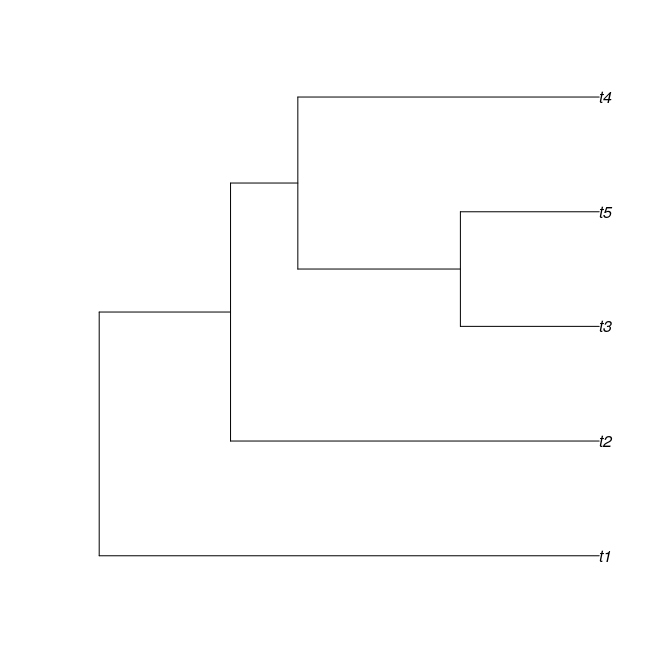
\includegraphics{mbd_vignette_files/figure-latex/unnamed-chunk-5-1.pdf}

\hypertarget{b-operator}{%
\subsubsection{B operator}\label{b-operator}}

The \(B^{k, k + b}\) operator, acting on the branching times, is built in a similar way.
The main difference is that \(b\) births are given and are observable on the tree.
If \(b = 1\) the transition can be explained by both speciation processes. They
are, though, mutually exclusive, as each of them has a probability proportional
to \(dt\) and each term of higher order is negligible.

\[
B^{k,k + b}_{m,n} = \lambda k \delta_{m,n} \delta_{b,1} + \nu N^{k,k + b}_{m,n}
\]

\hypertarget{b-operator-implementation}{%
\paragraph{B operator: Implementation}\label{b-operator-implementation}}

The \(B^{k, k + b}\) matrix can be created using

\begin{Shaded}
\begin{Highlighting}[]
\NormalTok{b <-}\StringTok{ }\DecValTok{1}
\NormalTok{b_matrix <-}\StringTok{ }\NormalTok{mbd}\OperatorTok{:::}\KeywordTok{create_b}\NormalTok{(}\DataTypeTok{pars =}\NormalTok{ pars, }\DataTypeTok{lx =}\NormalTok{ lx, }\DataTypeTok{k =}\NormalTok{ k, }\DataTypeTok{b =}\NormalTok{ b)}
\NormalTok{b_matrix}
\CommentTok{#>       [,1]  [,2]   [,3]    [,4]     [,5]      [,6]       [,7]       [,8]}
\CommentTok{#>  [1,] 0.58 0.000 0.0000 0.00000 0.000000 0.0000000 0.00000000 0.00000000}
\CommentTok{#>  [2,] 0.04 0.562 0.0000 0.00000 0.000000 0.0000000 0.00000000 0.00000000}
\CommentTok{#>  [3,] 0.00 0.054 0.5458 0.00000 0.000000 0.0000000 0.00000000 0.00000000}
\CommentTok{#>  [4,] 0.00 0.004 0.0648 0.53122 0.000000 0.0000000 0.00000000 0.00000000}
\CommentTok{#>  [5,] 0.00 0.000 0.0090 0.07290 0.518098 0.0000000 0.00000000 0.00000000}
\CommentTok{#>  [6,] 0.00 0.000 0.0004 0.01458 0.078732 0.5062882 0.00000000 0.00000000}
\CommentTok{#>  [7,] 0.00 0.000 0.0000 0.00126 0.020412 0.0826686 0.49565938 0.00000000}
\CommentTok{#>  [8,] 0.00 0.000 0.0000 0.00004 0.002592 0.0262440 0.08503056 0.48609344}
\CommentTok{#>  [9,] 0.00 0.000 0.0000 0.00000 0.000162 0.0043740 0.03188646 0.08609344}
\CommentTok{#> [10,] 0.00 0.000 0.0000 0.00000 0.000004 0.0004050 0.00656100 0.03720087}
\CommentTok{#>             [,9]     [,10]}
\CommentTok{#>  [1,] 0.00000000 0.0000000}
\CommentTok{#>  [2,] 0.00000000 0.0000000}
\CommentTok{#>  [3,] 0.00000000 0.0000000}
\CommentTok{#>  [4,] 0.00000000 0.0000000}
\CommentTok{#>  [5,] 0.00000000 0.0000000}
\CommentTok{#>  [6,] 0.00000000 0.0000000}
\CommentTok{#>  [7,] 0.00000000 0.0000000}
\CommentTok{#>  [8,] 0.00000000 0.0000000}
\CommentTok{#>  [9,] 0.47748410 0.0000000}
\CommentTok{#> [10,] 0.08609344 0.4697357}
\end{Highlighting}
\end{Shaded}

We can verify that the entries respect our definition:

\begin{Shaded}
\begin{Highlighting}[]
\CommentTok{# m < n}
\NormalTok{testthat}\OperatorTok{::}\KeywordTok{expect_true}\NormalTok{(}
  \KeywordTok{all}\NormalTok{(b_matrix[}\KeywordTok{upper.tri}\NormalTok{(b_matrix, }\DataTypeTok{diag =} \OtherTok{FALSE}\NormalTok{)] }\OperatorTok{==}\StringTok{ }\DecValTok{0}\NormalTok{)}
\NormalTok{)}
\CommentTok{# m >= n}
\ControlFlowTok{for}\NormalTok{ (m }\ControlFlowTok{in} \DecValTok{0}\OperatorTok{:}\NormalTok{lx) \{}
  \ControlFlowTok{for}\NormalTok{ (n }\ControlFlowTok{in} \DecValTok{0}\OperatorTok{:}\NormalTok{m) \{}
\NormalTok{    a <-}\StringTok{ }\NormalTok{m }\OperatorTok{-}\StringTok{ }\NormalTok{n}
\NormalTok{    j <-}\StringTok{ }\DecValTok{0}\OperatorTok{:}\KeywordTok{min}\NormalTok{(m }\OperatorTok{-}\StringTok{ }\NormalTok{n, k)}
\NormalTok{    entry_m_n <-}\StringTok{ }
\StringTok{      }\NormalTok{(m }\OperatorTok{==}\StringTok{ }\NormalTok{n) }\OperatorTok{*}\StringTok{ }\NormalTok{(b }\OperatorTok{==}\StringTok{ }\DecValTok{1}\NormalTok{) }\OperatorTok{*}\StringTok{ }\NormalTok{lambda }\OperatorTok{*}\StringTok{ }\NormalTok{k }\OperatorTok{+}
\StringTok{      }\NormalTok{nu }\OperatorTok{*}
\StringTok{      }\KeywordTok{choose}\NormalTok{(k, b) }\OperatorTok{*}\StringTok{ }\NormalTok{q }\OperatorTok{^}\StringTok{ }\NormalTok{b }\OperatorTok{*}
\StringTok{      }\NormalTok{(}\DecValTok{1} \OperatorTok{-}\StringTok{ }\NormalTok{q) }\OperatorTok{^}\StringTok{ }\NormalTok{(k }\OperatorTok{-}\StringTok{ }\NormalTok{b }\OperatorTok{+}\StringTok{ }\NormalTok{m) }\OperatorTok{*}
\StringTok{      }\NormalTok{q }\OperatorTok{^}\StringTok{ }\NormalTok{a }\OperatorTok{*}\StringTok{ }
\StringTok{      }\NormalTok{(}\DecValTok{1} \OperatorTok{-}\StringTok{ }\NormalTok{q) }\OperatorTok{^}\StringTok{ }\NormalTok{(}\OperatorTok{-}\DecValTok{2} \OperatorTok{*}\StringTok{ }\NormalTok{a) }\OperatorTok{*}
\StringTok{      }\KeywordTok{sum}\NormalTok{(}
        \DecValTok{2} \OperatorTok{^}\StringTok{ }\NormalTok{j }\OperatorTok{*}\StringTok{ }\KeywordTok{choose}\NormalTok{(k }\OperatorTok{-}\StringTok{ }\NormalTok{b, j) }\OperatorTok{*}\StringTok{ }\KeywordTok{choose}\NormalTok{(m }\OperatorTok{-}\StringTok{ }\NormalTok{a, a }\OperatorTok{-}\StringTok{ }\NormalTok{j)}
\NormalTok{      )}
\NormalTok{    testthat}\OperatorTok{::}\KeywordTok{expect_equal}\NormalTok{(}
\NormalTok{      entry_m_n,}
\NormalTok{      b_matrix[m }\OperatorTok{+}\StringTok{ }\DecValTok{1}\NormalTok{, n }\OperatorTok{+}\StringTok{ }\DecValTok{1}\NormalTok{]}
\NormalTok{    )}
\NormalTok{  \}}
\NormalTok{\}}
\end{Highlighting}
\end{Shaded}

\hypertarget{implementation-problems}{%
\section{Implementation problems}\label{implementation-problems}}

The goal of this section is to expose issues in the mbd likelihood computation
due to weird probabilities.

\hypertarget{negative-probabilities-in-the-q-vector}{%
\subsection{Negative Probabilities in the Q-vector}\label{negative-probabilities-in-the-q-vector}}

First we set the parameter that expose the problem.

\begin{Shaded}
\begin{Highlighting}[]
\NormalTok{brts <-}\StringTok{ }\KeywordTok{c}\NormalTok{(}\DecValTok{10}\NormalTok{, }\DecValTok{9}\NormalTok{, }\DecValTok{7}\NormalTok{, }\DecValTok{6}\NormalTok{, }\DecValTok{5}\NormalTok{) }\CommentTok{# branching times}
\NormalTok{pars <-}\StringTok{ }\KeywordTok{c}\NormalTok{(}\DecValTok{2}\NormalTok{, }\FloatTok{0.05}\NormalTok{, }\FloatTok{1.00}\NormalTok{, }\FloatTok{0.1}\NormalTok{) }\CommentTok{# mbd parameters = c(lambda, mu, nu, q)}
\NormalTok{n_}\DecValTok{0}\NormalTok{ <-}\StringTok{ }\DecValTok{2} \CommentTok{# starting species}
\NormalTok{cond <-}\StringTok{ }\DecValTok{1} \CommentTok{# conditioning? 1 is yes, 0 is no.}
\NormalTok{tips_interval <-}\StringTok{ }\KeywordTok{c}\NormalTok{(n_}\DecValTok{0} \OperatorTok{*}\StringTok{ }\NormalTok{(cond }\OperatorTok{>}\StringTok{ }\DecValTok{0}\NormalTok{), }\OtherTok{Inf}\NormalTok{) }\CommentTok{# how many tips are allowed in tree?}
\NormalTok{lx <-}\StringTok{ }\DecValTok{200} \CommentTok{# dimension of the transition matrix}
\NormalTok{abstol <-}\StringTok{ }\FloatTok{1e-16} \CommentTok{# absolute tolerance for ode}
\NormalTok{reltol <-}\StringTok{ }\FloatTok{1e-10} \CommentTok{# relative tolerance for ode}
\end{Highlighting}
\end{Shaded}

Then we try to calculate the likelihood with a given \link{ode} method. In this
first try we use ``ode45''.

\begin{Shaded}
\begin{Highlighting}[]
\NormalTok{methode <-}\StringTok{ "ode45"} \CommentTok{# ode method}
\NormalTok{loglik <-}\StringTok{ }\KeywordTok{mbd_loglik}\NormalTok{(}
  \DataTypeTok{pars =}\NormalTok{ pars,}
  \DataTypeTok{brts =}\NormalTok{ brts,}
  \DataTypeTok{n_0 =}\NormalTok{ n_}\DecValTok{0}\NormalTok{,}
  \DataTypeTok{cond =}\NormalTok{ cond,}
  \DataTypeTok{tips_interval =}\NormalTok{ tips_interval,}
  \DataTypeTok{lx =}\NormalTok{ lx,}
  \DataTypeTok{methode =}\NormalTok{ methode,}
  \DataTypeTok{abstol =}\NormalTok{ abstol,}
  \DataTypeTok{reltol =}\NormalTok{ reltol,}
  \DataTypeTok{debug_mode =} \OtherTok{TRUE}
\NormalTok{)}
\CommentTok{#>            Q0            Q1            Q2            Q3            Q4 }
\CommentTok{#>  2.386705e-42  2.872139e-41  1.871514e-40  8.752920e-40  3.288811e-39 }
\CommentTok{#>            Q5            Q6            Q7            Q8            Q9 }
\CommentTok{#>  1.054295e-38  2.992022e-38  7.705239e-38  1.832512e-37  4.077445e-37 }
\CommentTok{#>           Q10           Q11           Q12           Q13           Q14 }
\CommentTok{#>  8.572819e-37  1.716472e-36  3.293342e-36  6.086001e-36  1.087797e-35 }
\CommentTok{#>           Q15           Q16           Q17           Q18           Q19 }
\CommentTok{#>  1.887176e-35  3.187275e-35  5.253812e-35  8.470909e-35  1.338483e-34 }
\CommentTok{#>           Q20           Q21           Q22           Q23           Q24 }
\CommentTok{#>  2.076092e-34  3.165679e-34  4.751560e-34  7.028372e-34  1.025579e-33 }
\CommentTok{#>           Q25           Q26           Q27           Q28           Q29 }
\CommentTok{#>  1.477679e-33  2.104012e-33  2.962782e-33  4.128863e-33  5.697831e-33 }
\CommentTok{#>           Q30           Q31           Q32           Q33           Q34 }
\CommentTok{#>  7.790809e-33  1.056025e-32  1.419682e-32  1.893748e-32  2.507512e-32 }
\CommentTok{#>           Q35           Q36           Q37           Q38           Q39 }
\CommentTok{#>  3.296970e-32  4.306137e-32  5.588563e-32  7.209101e-32  9.245936e-32 }
\CommentTok{#>           Q40           Q41           Q42           Q43           Q44 }
\CommentTok{#>  1.179292e-31  1.496228e-31  1.888762e-31  2.372751e-31  2.966938e-31 }
\CommentTok{#>           Q45           Q46           Q47           Q48           Q49 }
\CommentTok{#>  3.693407e-31  4.578090e-31  5.651342e-31  6.948591e-31  8.511060e-31 }
\CommentTok{#>           Q50           Q51           Q52           Q53           Q54 }
\CommentTok{#>  1.038658e-30  1.263050e-30  1.530672e-30  1.848877e-30  2.226114e-30 }
\CommentTok{#>           Q55           Q56           Q57           Q58           Q59 }
\CommentTok{#>  2.672059e-30  3.197778e-30  3.815889e-30  4.540757e-30  5.388698e-30 }
\CommentTok{#>           Q60           Q61           Q62           Q63           Q64 }
\CommentTok{#>  6.378208e-30  7.530213e-30  8.868347e-30  1.041925e-29  1.221290e-29 }
\CommentTok{#>           Q65           Q66           Q67           Q68           Q69 }
\CommentTok{#>  1.428296e-29  1.666721e-29  1.940793e-29  2.255238e-29  2.615332e-29 }
\CommentTok{#>           Q70           Q71           Q72           Q73           Q74 }
\CommentTok{#>  3.026955e-29  3.496652e-29  4.031694e-29  4.640154e-29  5.330976e-29 }
\CommentTok{#>           Q75           Q76           Q77           Q78           Q79 }
\CommentTok{#>  6.114063e-29  7.000360e-29  8.001953e-29  9.132170e-29  1.040569e-28 }
\CommentTok{#>           Q80           Q81           Q82           Q83           Q84 }
\CommentTok{#>  1.183867e-28  1.344885e-28  1.525572e-28  1.728064e-28  1.954703e-28 }
\CommentTok{#>           Q85           Q86           Q87           Q88           Q89 }
\CommentTok{#>  2.208049e-28  2.490902e-28  2.806321e-28  3.157641e-28  3.548500e-28 }
\CommentTok{#>           Q90           Q91           Q92           Q93           Q94 }
\CommentTok{#>  3.982860e-28  4.465029e-28  4.999693e-28  5.591941e-28  6.247297e-28 }
\CommentTok{#>           Q95           Q96           Q97           Q98           Q99 }
\CommentTok{#>  6.971750e-28  7.771790e-28  8.654441e-28  9.627304e-28  1.069859e-27 }
\CommentTok{#>          Q100          Q101          Q102          Q103          Q104 }
\CommentTok{#>  1.187719e-27  1.317266e-27  1.459534e-27  1.615637e-27  1.786774e-27 }
\CommentTok{#>          Q105          Q106          Q107          Q108          Q109 }
\CommentTok{#>  1.974236e-27  2.179411e-27  2.403792e-27  2.648982e-27  2.916703e-27 }
\CommentTok{#>          Q110          Q111          Q112          Q113          Q114 }
\CommentTok{#>  3.208800e-27  3.527254e-27  3.874187e-27  4.251870e-27  4.662736e-27 }
\CommentTok{#>          Q115          Q116          Q117          Q118          Q119 }
\CommentTok{#>  5.109386e-27  5.594601e-27  6.121353e-27  6.692814e-27  7.312374e-27 }
\CommentTok{#>          Q120          Q121          Q122          Q123          Q124 }
\CommentTok{#>  7.983644e-27  8.710478e-27  9.496982e-27  1.034753e-26  1.126678e-26 }
\CommentTok{#>          Q125          Q126          Q127          Q128          Q129 }
\CommentTok{#>  1.225968e-26  1.333151e-26  1.448786e-26  1.573469e-26  1.707833e-26 }
\CommentTok{#>          Q130          Q131          Q132          Q133          Q134 }
\CommentTok{#>  1.852549e-26  2.008328e-26  2.175928e-26  2.356148e-26  2.549838e-26 }
\CommentTok{#>          Q135          Q136          Q137          Q138          Q139 }
\CommentTok{#>  2.757898e-26  2.981281e-26  3.220993e-26  3.478103e-26  3.753738e-26 }
\CommentTok{#>          Q140          Q141          Q142          Q143          Q144 }
\CommentTok{#>  4.049091e-26  4.365424e-26  4.704068e-26  5.066430e-26  5.453994e-26 }
\CommentTok{#>          Q145          Q146          Q147          Q148          Q149 }
\CommentTok{#>  5.868327e-26  6.311082e-26  6.784003e-26  7.288927e-26  7.827789e-26 }
\CommentTok{#>          Q150          Q151          Q152          Q153          Q154 }
\CommentTok{#>  8.402631e-26  9.015599e-26  9.668955e-26  1.036508e-25  1.110647e-25 }
\CommentTok{#>          Q155          Q156          Q157          Q158          Q159 }
\CommentTok{#>  1.189577e-25  1.273574e-25  1.362930e-25  1.457949e-25  1.558953e-25 }
\CommentTok{#>          Q160          Q161          Q162          Q163          Q164 }
\CommentTok{#>  1.666280e-25  1.780283e-25  1.901334e-25  2.029822e-25  2.166156e-25 }
\CommentTok{#>          Q165          Q166          Q167          Q168          Q169 }
\CommentTok{#>  2.310766e-25  2.464100e-25  2.626629e-25  2.798848e-25  2.981272e-25 }
\CommentTok{#>          Q170          Q171          Q172          Q173          Q174 }
\CommentTok{#>  3.174442e-25  3.378926e-25  3.595317e-25  3.824234e-25  4.066326e-25 }
\CommentTok{#>          Q175          Q176          Q177          Q178          Q179 }
\CommentTok{#>  4.322273e-25  4.592784e-25  4.878600e-25  5.180503e-25  5.499271e-25 }
\CommentTok{#>          Q180          Q181          Q182          Q183          Q184 }
\CommentTok{#>  5.835870e-25  6.190750e-25  6.566363e-25  6.958314e-25  7.386493e-25 }
\CommentTok{#>          Q185          Q186          Q187          Q188          Q189 }
\CommentTok{#>  7.784215e-25  8.398844e-25  8.371672e-25  9.908013e-25  1.876117e-24 }
\CommentTok{#>          Q190          Q191          Q192          Q193          Q194 }
\CommentTok{#> -1.518500e-23  1.956700e-22 -2.022116e-21  1.931722e-20 -1.719248e-19 }
\CommentTok{#>          Q195          Q196          Q197          Q198          Q199 }
\CommentTok{#>  1.428091e-18 -1.099409e-17  7.730321e-17 -4.829781e-16  2.528322e-15 }
\CommentTok{#>          Q200 }
\CommentTok{#> -9.284857e-15}
\end{Highlighting}
\end{Shaded}

\includegraphics{mbd_vignette_files/figure-latex/unnamed-chunk-9-1.pdf}

\begin{verbatim}
#>            Q0            Q1            Q2            Q3            Q4 
#> -3.327841e-28 -4.004694e-27 -2.609497e-26 -1.220441e-25 -4.585671e-25 
#>            Q5            Q6            Q7            Q8            Q9 
#> -1.470030e-24 -4.171850e-24 -1.074360e-23 -2.555116e-23 -5.685283e-23 
#>           Q10           Q11           Q12           Q13           Q14 
#> -1.195329e-22 -2.393319e-22 -4.591987e-22 -8.485861e-22 -1.516742e-21 
#>           Q15           Q16           Q17           Q18           Q19 
#> -2.631336e-21 -4.444096e-21 -7.325520e-21 -1.181120e-20 -1.866281e-20 
#>           Q20           Q21           Q22           Q23           Q24 
#> -2.894747e-20 -4.413984e-20 -6.625217e-20 -9.799832e-20 -1.429990e-19 
#>           Q25           Q26           Q27           Q28           Q29 
#> -2.060364e-19 -2.933675e-19 -4.131080e-19 -5.756975e-19 -7.944626e-19 
#>           Q30           Q31           Q32           Q33           Q34 
#> -1.086292e-18 -1.472442e-18 -1.979497e-18 -2.640500e-18 -3.496286e-18 
#>           Q35           Q36           Q37           Q38           Q39 
#> -4.597047e-18 -6.004152e-18 -7.792271e-18 -1.005183e-17 -1.289184e-17 
#>           Q40           Q41           Q42           Q43           Q44 
#> -1.644317e-17 -2.086227e-17 -2.633548e-17 -3.308385e-17 -4.136875e-17 
#>           Q45           Q46           Q47           Q48           Q49 
#> -5.149808e-17 -6.383343e-17 -7.879806e-17 -9.688593e-17 -1.186718e-16 
#>           Q50           Q51           Q52           Q53           Q54 
#> -1.448227e-16 -1.761102e-16 -2.134254e-16 -2.577935e-16 -3.103925e-16 
#>           Q55           Q56           Q57           Q58           Q59 
#> -3.725718e-16 -4.458740e-16 -5.320588e-16 -6.331290e-16 -7.513594e-16 
#>           Q60           Q61           Q62           Q63           Q64 
#> -8.893292e-16 -1.049956e-15 -1.236536e-15 -1.452782e-15 -1.702874e-15 
#>           Q65           Q66           Q67           Q68           Q69 
#> -1.991509e-15 -2.323951e-15 -2.706095e-15 -3.144534e-15 -3.646622e-15 
#>           Q70           Q71           Q72           Q73           Q74 
#> -4.220558e-15 -4.875468e-15 -5.621491e-15 -6.469881e-15 -7.433112e-15 
#>           Q75           Q76           Q77           Q78           Q79 
#> -8.524989e-15 -9.760775e-15 -1.115732e-14 -1.273321e-14 -1.450891e-14 
#>           Q80           Q81           Q82           Q83           Q84 
#> -1.650695e-14 -1.875206e-14 -2.127142e-14 -2.409483e-14 -2.725490e-14 
#>           Q85           Q86           Q87           Q88           Q89 
#> -3.078737e-14 -3.473126e-14 -3.912922e-14 -4.402777e-14 -4.947762e-14 
#>           Q90           Q91           Q92           Q93           Q94 
#> -5.553400e-14 -6.225700e-14 -6.971195e-14 -7.796982e-14 -8.710761e-14 
#>           Q95           Q96           Q97           Q98           Q99 
#> -9.720884e-14 -1.083640e-13 -1.206710e-13 -1.342359e-13 -1.491731e-13 
#>          Q100          Q101          Q102          Q103          Q104 
#> -1.656065e-13 -1.836696e-13 -2.035065e-13 -2.252723e-13 -2.491343e-13 
#>          Q105          Q106          Q107          Q108          Q109 
#> -2.752726e-13 -3.038807e-13 -3.351667e-13 -3.693541e-13 -4.066831e-13 
#>          Q110          Q111          Q112          Q113          Q114 
#> -4.474109e-13 -4.918138e-13 -5.401875e-13 -5.928488e-13 -6.501368e-13 
#>          Q115          Q116          Q117          Q118          Q119 
#> -7.124143e-13 -7.800690e-13 -8.535153e-13 -9.331956e-13 -1.019582e-12 
#>          Q120          Q121          Q122          Q123          Q124 
#> -1.113179e-12 -1.214523e-12 -1.324188e-12 -1.442782e-12 -1.570955e-12 
#>          Q125          Q126          Q127          Q128          Q129 
#> -1.709397e-12 -1.858845e-12 -2.020078e-12 -2.193927e-12 -2.381274e-12 
#>          Q130          Q131          Q132          Q133          Q134 
#> -2.583054e-12 -2.800262e-12 -3.033950e-12 -3.285235e-12 -3.555303e-12 
#>          Q135          Q136          Q137          Q138          Q139 
#> -3.845406e-12 -4.156873e-12 -4.491110e-12 -4.849604e-12 -5.233929e-12 
#>          Q140          Q141          Q142          Q143          Q144 
#> -5.645748e-12 -6.086819e-12 -6.558998e-12 -7.064248e-12 -7.604638e-12 
#>          Q145          Q146          Q147          Q148          Q149 
#> -8.182353e-12 -8.799698e-12 -9.459103e-12 -1.016313e-11 -1.091448e-11 
#>          Q150          Q151          Q152          Q153          Q154 
#> -1.171600e-11 -1.257067e-11 -1.348166e-11 -1.445228e-11 -1.548603e-11 
#>          Q155          Q156          Q157          Q158          Q159 
#> -1.658657e-11 -1.775776e-11 -1.900367e-11 -2.032854e-11 -2.173687e-11 
#>          Q160          Q161          Q162          Q163          Q164 
#> -2.323335e-11 -2.482292e-11 -2.651076e-11 -2.830230e-11 -3.020325e-11 
#>          Q165          Q166          Q167          Q168          Q169 
#> -3.221958e-11 -3.435755e-11 -3.662374e-11 -3.902502e-11 -4.156861e-11 
#>          Q170          Q171          Q172          Q173          Q174 
#> -4.426203e-11 -4.711320e-11 -5.013039e-11 -5.332223e-11 -5.669779e-11 
#>          Q175          Q176          Q177          Q178          Q179 
#> -6.026652e-11 -6.403833e-11 -6.802352e-11 -7.223303e-11 -7.667769e-11 
#>          Q180          Q181          Q182          Q183          Q184 
#> -8.137097e-11 -8.631915e-11 -9.155643e-11 -9.702149e-11 -1.029917e-10 
#>          Q185          Q186          Q187          Q188          Q189 
#> -1.085372e-10 -1.171071e-10 -1.167283e-10 -1.381499e-10 -2.615916e-10 
#>          Q190          Q191          Q192          Q193          Q194 
#>  2.117282e-09 -2.728275e-08  2.819486e-07 -2.693448e-06  2.397191e-05 
#>          Q195          Q196          Q197          Q198          Q199 
#> -1.991222e-04  1.532933e-03 -1.077858e-02  6.734282e-02 -3.525301e-01 
#>          Q200 
#>  1.294611e+00
#> [1] 2.00 0.05 1.00 0.10
#> [1]  1.000000e+00  1.640778e-02  2.625566e-02  3.302733e+01  6.545368e+01
#> [6] -1.394325e+14
#> Warning in log(likelihood): Si è prodotto un NaN
#> Warning in log(C): Si è prodotto un NaN
\end{verbatim}

\includegraphics{mbd_vignette_files/figure-latex/unnamed-chunk-9-2.pdf}

The same problem appears if we use ``lsodes'':

\begin{Shaded}
\begin{Highlighting}[]
\NormalTok{methode <-}\StringTok{ "lsodes"} \CommentTok{# ode method}
\NormalTok{loglik <-}\StringTok{ }\KeywordTok{mbd_loglik}\NormalTok{(}
  \DataTypeTok{pars =}\NormalTok{ pars,}
  \DataTypeTok{brts =}\NormalTok{ brts,}
  \DataTypeTok{n_0 =}\NormalTok{ n_}\DecValTok{0}\NormalTok{,}
  \DataTypeTok{cond =}\NormalTok{ cond,}
  \DataTypeTok{tips_interval =}\NormalTok{ tips_interval,}
  \DataTypeTok{lx =}\NormalTok{ lx,}
  \DataTypeTok{methode =}\NormalTok{ methode,}
  \DataTypeTok{abstol =}\NormalTok{ abstol,}
  \DataTypeTok{reltol =}\NormalTok{ reltol,}
  \DataTypeTok{debug_mode =} \OtherTok{TRUE}
\NormalTok{)}
\CommentTok{#>            Q0            Q1            Q2            Q3            Q4 }
\CommentTok{#>  5.490134e-38  6.617954e-37  4.319601e-36  2.023645e-35  7.616396e-35 }
\CommentTok{#>            Q5            Q6            Q7            Q8            Q9 }
\CommentTok{#>  2.445683e-34  6.952302e-34  1.793387e-33  4.272256e-33  9.521811e-33 }
\CommentTok{#>           Q10           Q11           Q12           Q13           Q14 }
\CommentTok{#>  2.005276e-32  4.021655e-32  7.728957e-32  1.430640e-31  2.561290e-31 }
\CommentTok{#>           Q15           Q16           Q17           Q18           Q19 }
\CommentTok{#>  4.450763e-31  7.529237e-31  1.243122e-30  2.007592e-30  3.177337e-30 }
\CommentTok{#>           Q20           Q21           Q22           Q23           Q24 }
\CommentTok{#>  4.936281e-30  7.539133e-30  1.133419e-29  1.679219e-29  2.454250e-29 }
\CommentTok{#>           Q25           Q26           Q27           Q28           Q29 }
\CommentTok{#>  3.541805e-29  5.051123e-29  7.124123e-29  9.943807e-29  1.374425e-28 }
\CommentTok{#>           Q30           Q31           Q32           Q33           Q34 }
\CommentTok{#>  1.882270e-28  2.555411e-28  3.440837e-28  4.597085e-28  6.096651e-28 }
\CommentTok{#>           Q35           Q36           Q37           Q38           Q39 }
\CommentTok{#>  8.028670e-28  1.050257e-27  1.365168e-27  1.763767e-27  2.265620e-27 }
\CommentTok{#>           Q40           Q41           Q42           Q43           Q44 }
\CommentTok{#>  2.894198e-27  3.677681e-27  4.649670e-27  5.850138e-27  7.326806e-27 }
\CommentTok{#>           Q45           Q46           Q47           Q48           Q49 }
\CommentTok{#>  9.135585e-27  1.134131e-26  1.402188e-26  1.727009e-26  2.118638e-26 }
\CommentTok{#>           Q50           Q51           Q52           Q53           Q54 }
\CommentTok{#>  2.589591e-26  3.155026e-26  3.829657e-26  4.633265e-26  5.587960e-26 }
\CommentTok{#>           Q55           Q56           Q57           Q58           Q59 }
\CommentTok{#>  6.718865e-26  8.054547e-26  9.628985e-26  1.147986e-25  1.365071e-25 }
\CommentTok{#>           Q60           Q61           Q62           Q63           Q64 }
\CommentTok{#>  1.619127e-25  1.915838e-25  2.261692e-25  2.664095e-25  3.131488e-25 }
\CommentTok{#>           Q65           Q66           Q67           Q68           Q69 }
\CommentTok{#>  3.673355e-25  4.294835e-25  5.017208e-25  5.841915e-25  6.801959e-25 }
\CommentTok{#>           Q70           Q71           Q72           Q73           Q74 }
\CommentTok{#>  7.947133e-25  9.218518e-25  1.068843e-24  1.238092e-24  1.432693e-24 }
\CommentTok{#>           Q75           Q76           Q77           Q78           Q79 }
\CommentTok{#>  1.656306e-24  1.912450e-24  2.177708e-24  2.490714e-24  2.825789e-24 }
\CommentTok{#>           Q80           Q81           Q82           Q83           Q84 }
\CommentTok{#>  3.229128e-24  3.665229e-24  4.177147e-24  4.718466e-24  5.323901e-24 }
\CommentTok{#>           Q85           Q86           Q87           Q88           Q89 }
\CommentTok{#>  6.007384e-24  6.657478e-24  7.405734e-24  8.319493e-24  9.256379e-24 }
\CommentTok{#>           Q90           Q91           Q92           Q93           Q94 }
\CommentTok{#>  1.034909e-23  1.146954e-23  1.232265e-23  1.360846e-23  1.515611e-23 }
\CommentTok{#>           Q95           Q96           Q97           Q98           Q99 }
\CommentTok{#>  1.637152e-23  1.772108e-23  1.956200e-23  2.125077e-23  2.028131e-23 }
\CommentTok{#>          Q100          Q101          Q102          Q103          Q104 }
\CommentTok{#>  1.985517e-23  2.119609e-23  2.180061e-23  2.352452e-23  2.481116e-23 }
\CommentTok{#>          Q105          Q106          Q107          Q108          Q109 }
\CommentTok{#>  2.469415e-23  2.137799e-23  2.239988e-23  2.037505e-23  9.029818e-24 }
\CommentTok{#>          Q110          Q111          Q112          Q113          Q114 }
\CommentTok{#> -2.343426e-23 -6.289401e-23 -1.066792e-22 -1.315595e-22 -1.715846e-22 }
\CommentTok{#>          Q115          Q116          Q117          Q118          Q119 }
\CommentTok{#> -1.995649e-22 -2.207948e-22 -2.455742e-22 -3.376673e-22 -4.419819e-22 }
\CommentTok{#>          Q120          Q121          Q122          Q123          Q124 }
\CommentTok{#> -4.909495e-22 -6.223840e-22 -7.348824e-22 -8.250413e-22 -9.934267e-22 }
\CommentTok{#>          Q125          Q126          Q127          Q128          Q129 }
\CommentTok{#> -1.179479e-21 -1.369130e-21 -1.598658e-21 -1.844679e-21 -2.158036e-21 }
\CommentTok{#>          Q130          Q131          Q132          Q133          Q134 }
\CommentTok{#> -2.506976e-21 -2.854526e-21 -3.267536e-21 -3.724944e-21 -4.228161e-21 }
\CommentTok{#>          Q135          Q136          Q137          Q138          Q139 }
\CommentTok{#> -4.779159e-21 -5.367661e-21 -5.999345e-21 -6.700446e-21 -7.487126e-21 }
\CommentTok{#>          Q140          Q141          Q142          Q143          Q144 }
\CommentTok{#> -8.358473e-21 -9.018277e-21 -1.004300e-20 -1.115539e-20 -1.235442e-20 }
\CommentTok{#>          Q145          Q146          Q147          Q148          Q149 }
\CommentTok{#> -1.364012e-20 -1.500714e-20 -1.645192e-20 -1.802272e-20 -1.972548e-20 }
\CommentTok{#>          Q150          Q151          Q152          Q153          Q154 }
\CommentTok{#> -2.117500e-20 -2.307517e-20 -2.502988e-20 -2.702805e-20 -2.913757e-20 }
\CommentTok{#>          Q155          Q156          Q157          Q158          Q159 }
\CommentTok{#> -3.135636e-20 -3.368133e-20 -3.611455e-20 -3.866313e-20 -4.134210e-20 }
\CommentTok{#>          Q160          Q161          Q162          Q163          Q164 }
\CommentTok{#> -4.417390e-20 -4.718237e-20 -5.038882e-20 -5.380622e-20 -5.743807e-20 }
\CommentTok{#>          Q165          Q166          Q167          Q168          Q169 }
\CommentTok{#> -6.127745e-20 -6.530996e-20 -6.951685e-20 -7.387930e-20 -7.838143e-20 }
\CommentTok{#>          Q170          Q171          Q172          Q173          Q174 }
\CommentTok{#> -8.301251e-20 -8.776735e-20 -9.264498e-20 -9.764931e-20 -1.027875e-19 }
\CommentTok{#>          Q175          Q176          Q177          Q178          Q179 }
\CommentTok{#> -1.080916e-19 -1.141407e-19 -1.204238e-19 -1.262303e-19 -1.330049e-19 }
\CommentTok{#>          Q180          Q181          Q182          Q183          Q184 }
\CommentTok{#> -1.400594e-19 -1.466820e-19 -1.535261e-19 -1.605980e-19 -1.679026e-19 }
\CommentTok{#>          Q185          Q186          Q187          Q188          Q189 }
\CommentTok{#> -1.754442e-19 -1.832284e-19 -1.912625e-19 -1.995586e-19 -2.081419e-19 }
\CommentTok{#>          Q190          Q191          Q192          Q193          Q194 }
\CommentTok{#> -2.170275e-19 -2.262377e-19 -2.358089e-19 -2.457163e-19 -2.559378e-19 }
\CommentTok{#>          Q195          Q196          Q197          Q198          Q199 }
\CommentTok{#> -2.664581e-19 -2.771677e-19 -2.879798e-19 -2.988336e-19 -3.095158e-19 }
\CommentTok{#>          Q200 }
\CommentTok{#> -3.146693e-19}
\end{Highlighting}
\end{Shaded}

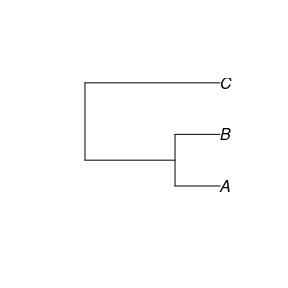
\includegraphics{mbd_vignette_files/figure-latex/unnamed-chunk-10-1.pdf}

\begin{verbatim}
#>            Q0            Q1            Q2            Q3            Q4 
#> -8.038885e-21 -9.690288e-20 -6.324943e-19 -2.963107e-18 -1.115225e-17 
#>            Q5            Q6            Q7            Q8            Q9 
#> -3.581073e-17 -1.017985e-16 -2.625954e-16 -6.255618e-16 -1.394224e-15 
#>           Q10           Q11           Q12           Q13           Q14 
#> -2.936210e-15 -5.888677e-15 -1.131706e-14 -2.094803e-14 -3.750349e-14 
#>           Q15           Q16           Q17           Q18           Q19 
#> -6.516995e-14 -1.102463e-13 -1.820232e-13 -2.939601e-13 -4.652391e-13 
#>           Q20           Q21           Q22           Q23           Q24 
#> -7.227911e-13 -1.103912e-12 -1.659600e-12 -2.458784e-12 -3.593616e-12 
#>           Q25           Q26           Q27           Q28           Q29 
#> -5.186060e-12 -7.396067e-12 -1.043144e-11 -1.456014e-11 -2.012490e-11 
#>           Q30           Q31           Q32           Q33           Q34 
#> -2.756099e-11 -3.741740e-11 -5.038219e-11 -6.731246e-11 -8.926974e-11 
#>           Q35           Q36           Q37           Q38           Q39 
#> -1.175592e-10 -1.537831e-10 -1.998936e-10 -2.582583e-10 -3.317416e-10 
#>           Q40           Q41           Q42           Q43           Q44 
#> -4.237807e-10 -5.385015e-10 -6.808244e-10 -8.566019e-10 -1.072822e-09 
#>           Q45           Q46           Q47           Q48           Q49 
#> -1.337671e-09 -1.660643e-09 -2.053143e-09 -2.528760e-09 -3.102199e-09 
#>           Q50           Q51           Q52           Q53           Q54 
#> -3.791789e-09 -4.619723e-09 -5.607546e-09 -6.784222e-09 -8.182127e-09 
#>           Q55           Q56           Q57           Q58           Q59 
#> -9.838046e-09 -1.179381e-08 -1.409917e-08 -1.680930e-08 -1.998794e-08 
#>           Q60           Q61           Q62           Q63           Q64 
#> -2.370794e-08 -2.805251e-08 -3.311664e-08 -3.900880e-08 -4.585258e-08 
#>           Q65           Q66           Q67           Q68           Q69 
#> -5.378681e-08 -6.288678e-08 -7.346408e-08 -8.553979e-08 -9.959716e-08 
#>           Q70           Q71           Q72           Q73           Q74 
#> -1.163653e-07 -1.349814e-07 -1.565044e-07 -1.812866e-07 -2.097810e-07 
#>           Q75           Q76           Q77           Q78           Q79 
#> -2.425233e-07 -2.800290e-07 -3.188693e-07 -3.647008e-07 -4.137639e-07 
#>           Q80           Q81           Q82           Q83           Q84 
#> -4.728226e-07 -5.366783e-07 -6.116355e-07 -6.908977e-07 -7.795481e-07 
#>           Q85           Q86           Q87           Q88           Q89 
#> -8.796265e-07 -9.748160e-07 -1.084379e-06 -1.218175e-06 -1.355358e-06 
#>           Q90           Q91           Q92           Q93           Q94 
#> -1.515357e-06 -1.679419e-06 -1.804334e-06 -1.992608e-06 -2.219222e-06 
#>           Q95           Q96           Q97           Q98           Q99 
#> -2.397187e-06 -2.594795e-06 -2.864351e-06 -3.111628e-06 -2.969675e-06 
#>          Q100          Q101          Q102          Q103          Q104 
#> -2.907277e-06 -3.103621e-06 -3.192137e-06 -3.444560e-06 -3.632955e-06 
#>          Q105          Q106          Q107          Q108          Q109 
#> -3.615821e-06 -3.130255e-06 -3.279885e-06 -2.983401e-06 -1.322184e-06 
#>          Q110          Q111          Q112          Q113          Q114 
#>  3.431343e-06  9.209207e-06  1.562042e-05  1.926349e-05  2.512415e-05 
#>          Q115          Q116          Q117          Q118          Q119 
#>  2.922114e-05  3.232970e-05  3.595801e-05  4.944267e-05  6.471686e-05 
#>          Q120          Q121          Q122          Q123          Q124 
#>  7.188690e-05  9.113209e-05  1.076046e-04  1.208060e-04  1.454617e-04 
#>          Q125          Q126          Q127          Q128          Q129 
#>  1.727043e-04  2.004738e-04  2.340823e-04  2.701057e-04  3.159888e-04 
#>          Q130          Q131          Q132          Q133          Q134 
#>  3.670820e-04  4.179717e-04  4.784464e-04  5.454221e-04  6.191052e-04 
#>          Q135          Q136          Q137          Q138          Q139 
#>  6.997846e-04  7.859556e-04  8.784494e-04  9.811076e-04  1.096297e-03 
#>          Q140          Q141          Q142          Q143          Q144 
#>  1.223883e-03  1.320494e-03  1.470538e-03  1.633419e-03  1.808986e-03 
#>          Q145          Q146          Q147          Q148          Q149 
#>  1.997244e-03  2.197408e-03  2.408960e-03  2.638963e-03  2.888289e-03 
#>          Q150          Q151          Q152          Q153          Q154 
#>  3.100532e-03  3.378764e-03  3.664981e-03  3.957561e-03  4.266446e-03 
#>          Q155          Q156          Q157          Q158          Q159 
#>  4.591331e-03  4.931763e-03  5.288045e-03  5.661219e-03  6.053485e-03 
#>          Q160          Q161          Q162          Q163          Q164 
#>  6.468129e-03  6.908642e-03  7.378143e-03  7.878534e-03  8.410324e-03 
#>          Q165          Q166          Q167          Q168          Q169 
#>  8.972503e-03  9.562960e-03  1.017895e-02  1.081772e-02  1.147694e-02 
#>          Q170          Q171          Q172          Q173          Q174 
#>  1.215504e-02  1.285127e-02  1.356547e-02  1.429822e-02  1.505059e-02 
#>          Q175          Q176          Q177          Q178          Q179 
#>  1.582723e-02  1.671297e-02  1.763296e-02  1.848317e-02  1.947514e-02 
#>          Q180          Q181          Q182          Q183          Q184 
#>  2.050809e-02  2.147780e-02  2.247995e-02  2.351544e-02  2.458501e-02 
#>          Q185          Q186          Q187          Q188          Q189 
#>  2.568927e-02  2.682908e-02  2.800546e-02  2.922022e-02  3.047701e-02 
#>          Q190          Q191          Q192          Q193          Q194 
#>  3.177809e-02  3.312667e-02  3.452814e-02  3.597882e-02  3.747549e-02 
#>          Q195          Q196          Q197          Q198          Q199 
#>  3.901593e-02  4.058407e-02  4.216722e-02  4.375648e-02  4.532061e-02 
#>          Q200 
#>  4.607520e-02
#> [1] 2.00 0.05 1.00 0.10
#> [1]  1.000000e+00  1.640778e-02  2.625566e-02  3.302733e+01  6.545367e+01
#> [6] -1.464242e+17
#> Warning in log(likelihood): Si è prodotto un NaN
#> Warning in log(C): Si è prodotto un NaN
\end{verbatim}

\includegraphics{mbd_vignette_files/figure-latex/unnamed-chunk-10-2.pdf}

And also with ``lsoda'':

\begin{Shaded}
\begin{Highlighting}[]
\NormalTok{methode <-}\StringTok{ "lsoda"} \CommentTok{# ode method}
\NormalTok{loglik <-}\StringTok{ }\KeywordTok{mbd_loglik}\NormalTok{(}
  \DataTypeTok{pars =}\NormalTok{ pars,}
  \DataTypeTok{brts =}\NormalTok{ brts,}
  \DataTypeTok{n_0 =}\NormalTok{ n_}\DecValTok{0}\NormalTok{,}
  \DataTypeTok{cond =}\NormalTok{ cond,}
  \DataTypeTok{tips_interval =}\NormalTok{ tips_interval,}
  \DataTypeTok{lx =}\NormalTok{ lx,}
  \DataTypeTok{methode =}\NormalTok{ methode,}
  \DataTypeTok{abstol =}\NormalTok{ abstol,}
  \DataTypeTok{reltol =}\NormalTok{ reltol,}
  \DataTypeTok{debug_mode =} \OtherTok{TRUE}
\NormalTok{)}
\CommentTok{#>            Q0            Q1            Q2            Q3            Q4 }
\CommentTok{#>  1.503891e-36  1.829705e-35  1.205207e-34  5.697061e-34  2.163237e-33 }
\CommentTok{#>            Q5            Q6            Q7            Q8            Q9 }
\CommentTok{#>  7.007032e-33  2.009019e-32  5.226304e-32  1.255417e-31  2.821022e-31 }
\CommentTok{#>           Q10           Q11           Q12           Q13           Q14 }
\CommentTok{#>  5.989146e-31  1.210731e-30  2.345124e-30  4.374496e-30  7.891527e-30 }
\CommentTok{#>           Q15           Q16           Q17           Q18           Q19 }
\CommentTok{#>  1.381638e-29  2.354628e-29  3.916079e-29  6.369937e-29  1.015317e-28 }
\CommentTok{#>           Q20           Q21           Q22           Q23           Q24 }
\CommentTok{#>  1.588454e-28  2.442819e-28  3.697555e-28  5.515003e-28  8.113945e-28 }
\CommentTok{#>           Q25           Q26           Q27           Q28           Q29 }
\CommentTok{#>  1.178623e-27  1.691749e-27  2.401276e-27  3.372793e-27  4.690818e-27 }
\CommentTok{#>           Q30           Q31           Q32           Q33           Q34 }
\CommentTok{#>  6.463460e-27  8.828046e-27  1.195787e-26  1.607029e-26  2.143626e-26 }
\CommentTok{#>           Q35           Q36           Q37           Q38           Q39 }
\CommentTok{#>  2.839175e-26  3.735112e-26  4.882278e-26  6.342762e-26  8.192041e-26 }
\CommentTok{#>           Q40           Q41           Q42           Q43           Q44 }
\CommentTok{#>  1.052146e-25  1.344113e-25  1.708320e-25  2.160574e-25  2.719705e-25 }
\CommentTok{#>           Q45           Q46           Q47           Q48           Q49 }
\CommentTok{#>  3.408072e-25  4.252130e-25  5.283080e-25  6.537609e-25  8.058720e-25 }
\CommentTok{#>           Q50           Q51           Q52           Q53           Q54 }
\CommentTok{#>  9.896673e-25  1.211005e-24  1.476696e-24  1.794634e-24  2.173949e-24 }
\CommentTok{#>           Q55           Q56           Q57           Q58           Q59 }
\CommentTok{#>  2.625175e-24  3.160437e-24  3.793653e-24  4.540777e-24  5.420046e-24 }
\CommentTok{#>           Q60           Q61           Q62           Q63           Q64 }
\CommentTok{#>  6.452273e-24  7.661152e-24  9.073614e-24  1.072022e-23  1.263558e-23 }
\CommentTok{#>           Q65           Q66           Q67           Q68           Q69 }
\CommentTok{#>  1.485878e-23  1.743397e-23  2.041084e-23  2.384530e-23  2.780000e-23 }
\CommentTok{#>           Q70           Q71           Q72           Q73           Q74 }
\CommentTok{#>  3.234523e-23  3.755984e-23  4.353188e-23  5.035932e-23  5.815201e-23 }
\CommentTok{#>           Q75           Q76           Q77           Q78           Q79 }
\CommentTok{#>  6.703210e-23  7.713549e-23  8.861094e-23  1.016256e-22  1.163648e-22 }
\CommentTok{#>           Q80           Q81           Q82           Q83           Q84 }
\CommentTok{#>  1.330313e-22  1.518548e-22  1.730787e-22  1.969791e-22  2.238620e-22 }
\CommentTok{#>           Q85           Q86           Q87           Q88           Q89 }
\CommentTok{#>  2.540657e-22  2.879508e-22  3.259470e-22  3.684408e-22  4.159239e-22 }
\CommentTok{#>           Q90           Q91           Q92           Q93           Q94 }
\CommentTok{#>  4.689403e-22  5.280902e-22  5.939201e-22  6.671579e-22  7.485313e-22 }
\CommentTok{#>           Q95           Q96           Q97           Q98           Q99 }
\CommentTok{#>  8.389059e-22  9.389128e-22  1.049684e-21  1.172203e-21  1.308150e-21 }
\CommentTok{#>          Q100          Q101          Q102          Q103          Q104 }
\CommentTok{#>  1.459424e-21  1.626380e-21  1.810220e-21  2.011101e-21  2.231818e-21 }
\CommentTok{#>          Q105          Q106          Q107          Q108          Q109 }
\CommentTok{#>  2.476808e-21  2.747300e-21  3.041933e-21  3.363050e-21  3.714195e-21 }
\CommentTok{#>          Q110          Q111          Q112          Q113          Q114 }
\CommentTok{#>  4.102120e-21  4.522372e-21  4.978876e-21  5.483913e-21  6.036297e-21 }
\CommentTok{#>          Q115          Q116          Q117          Q118          Q119 }
\CommentTok{#>  6.636654e-21  7.296008e-21  8.006876e-21  8.801529e-21  9.682717e-21 }
\CommentTok{#>          Q120          Q121          Q122          Q123          Q124 }
\CommentTok{#>  1.062181e-20  1.166299e-20  1.279494e-20  1.404540e-20  1.536412e-20 }
\CommentTok{#>          Q125          Q126          Q127          Q128          Q129 }
\CommentTok{#>  1.673868e-20  1.822782e-20  1.987999e-20  2.162132e-20  2.343950e-20 }
\CommentTok{#>          Q130          Q131          Q132          Q133          Q134 }
\CommentTok{#>  2.532309e-20  2.714021e-20  2.920703e-20  3.150817e-20  3.421824e-20 }
\CommentTok{#>          Q135          Q136          Q137          Q138          Q139 }
\CommentTok{#>  3.751751e-20  4.136306e-20  4.550973e-20  4.950321e-20  5.427336e-20 }
\CommentTok{#>          Q140          Q141          Q142          Q143          Q144 }
\CommentTok{#>  5.921246e-20  6.383793e-20  6.971910e-20  7.542663e-20  7.994462e-20 }
\CommentTok{#>          Q145          Q146          Q147          Q148          Q149 }
\CommentTok{#>  8.747101e-20  9.261006e-20  9.827954e-20  1.058553e-19  1.120198e-19 }
\CommentTok{#>          Q150          Q151          Q152          Q153          Q154 }
\CommentTok{#>  1.194669e-19  1.322036e-19  1.403488e-19  1.437257e-19  1.624796e-19 }
\CommentTok{#>          Q155          Q156          Q157          Q158          Q159 }
\CommentTok{#>  1.786446e-19  1.780062e-19  1.969077e-19  2.293755e-19  2.202769e-19 }
\CommentTok{#>          Q160          Q161          Q162          Q163          Q164 }
\CommentTok{#>  2.300290e-19  2.828319e-19  2.931973e-19  2.350142e-19  2.945520e-19 }
\CommentTok{#>          Q165          Q166          Q167          Q168          Q169 }
\CommentTok{#>  4.296589e-19  4.454669e-19  3.298122e-19  3.406950e-19  5.779180e-19 }
\CommentTok{#>          Q170          Q171          Q172          Q173          Q174 }
\CommentTok{#>  7.244816e-19  6.368677e-19  2.476326e-19  2.921732e-19  1.069790e-18 }
\CommentTok{#>          Q175          Q176          Q177          Q178          Q179 }
\CommentTok{#>  1.497904e-18  3.052888e-19 -4.154975e-19  1.610135e-18  2.443903e-18 }
\CommentTok{#>          Q180          Q181          Q182          Q183          Q184 }
\CommentTok{#> -6.166695e-19 -1.192860e-18  3.058863e-18  3.531345e-18 -4.732307e-19 }
\CommentTok{#>          Q185          Q186          Q187          Q188          Q189 }
\CommentTok{#> -8.827103e-19  1.666325e-18  2.217068e-18  1.327682e-18  6.003665e-19 }
\CommentTok{#>          Q190          Q191          Q192          Q193          Q194 }
\CommentTok{#>  2.439511e-18  5.134582e-18  1.923584e-18 -5.520623e-18  1.003915e-19 }
\CommentTok{#>          Q195          Q196          Q197          Q198          Q199 }
\CommentTok{#>  1.206280e-17  2.027194e-18 -8.801193e-18  5.505668e-18  2.138526e-17 }
\CommentTok{#>          Q200 }
\CommentTok{#>  1.200396e-17}
\end{Highlighting}
\end{Shaded}

\includegraphics{mbd_vignette_files/figure-latex/unnamed-chunk-11-1.pdf}

\begin{verbatim}
#>            Q0            Q1            Q2            Q3            Q4 
#>  2.072711e-20  2.521759e-19  1.661055e-18  7.851877e-18  2.981445e-17 
#>            Q5            Q6            Q7            Q8            Q9 
#>  9.657321e-17  2.768896e-16  7.203063e-16  1.730257e-15  3.888025e-15 
#>           Q10           Q11           Q12           Q13           Q14 
#>  8.254437e-15  1.668669e-14  3.232126e-14  6.029074e-14  1.087636e-13 
#>           Q15           Q16           Q17           Q18           Q19 
#>  1.904219e-13  3.245225e-13  5.397268e-13  8.779257e-13  1.399343e-12 
#>           Q20           Q21           Q22           Q23           Q24 
#>  2.189260e-12  3.366773e-12  5.096091e-12  7.600958e-12  1.118291e-11 
#>           Q25           Q26           Q27           Q28           Q29 
#>  1.624417e-11  2.331625e-11  3.309518e-11  4.648494e-11  6.465039e-11 
#>           Q30           Q31           Q32           Q33           Q34 
#>  8.908153e-11  1.216710e-10  1.648073e-10  2.214860e-10  2.954415e-10 
#>           Q35           Q36           Q37           Q38           Q39 
#>  3.913045e-10  5.147854e-10  6.728915e-10  8.741803e-10  1.129054e-09 
#>           Q40           Q41           Q42           Q43           Q44 
#>  1.450103e-09  1.852501e-09  2.354463e-09  2.977774e-09  3.748387e-09 
#>           Q45           Q46           Q47           Q48           Q49 
#>  4.697117e-09  5.860425e-09  7.281315e-09  9.010348e-09  1.110679e-08 
#>           Q50           Q51           Q52           Q53           Q54 
#>  1.363992e-08  1.669047e-08  2.035230e-08  2.473423e-08  2.996208e-08 
#>           Q55           Q56           Q57           Q58           Q59 
#>  3.618103e-08  4.355818e-08  5.228537e-08  6.258248e-08  7.470086e-08 
#>           Q60           Q61           Q62           Q63           Q64 
#>  8.892734e-08  1.055885e-07  1.250555e-07  1.477496e-07  1.741477e-07 
#>           Q65           Q66           Q67           Q68           Q69 
#>  2.047885e-07  2.402807e-07  2.813089e-07  3.286437e-07  3.831487e-07 
#>           Q70           Q71           Q72           Q73           Q74 
#>  4.457926e-07  5.176620e-07  5.999706e-07  6.940687e-07  8.014701e-07 
#>           Q75           Q76           Q77           Q78           Q79 
#>  9.238584e-07  1.063107e-06  1.221265e-06  1.400638e-06  1.603778e-06 
#>           Q80           Q81           Q82           Q83           Q84 
#>  1.833481e-06  2.092913e-06  2.385427e-06  2.714831e-06  3.085340e-06 
#>           Q85           Q86           Q87           Q88           Q89 
#>  3.501617e-06  3.968632e-06  4.492309e-06  5.077973e-06  5.732400e-06 
#>           Q90           Q91           Q92           Q93           Q94 
#>  6.463089e-06  7.278313e-06  8.185602e-06  9.194990e-06  1.031650e-05 
#>           Q95           Q96           Q97           Q98           Q99 
#>  1.156208e-05  1.294040e-05  1.446709e-05  1.615569e-05  1.802935e-05 
#>          Q100          Q101          Q102          Q103          Q104 
#>  2.011426e-05  2.241531e-05  2.494904e-05  2.771766e-05  3.075965e-05 
#>          Q105          Q106          Q107          Q108          Q109 
#>  3.413619e-05  3.786419e-05  4.192492e-05  4.635066e-05  5.119026e-05 
#>          Q110          Q111          Q112          Q113          Q114 
#>  5.653676e-05  6.232882e-05  6.862051e-05  7.558108e-05  8.319423e-05 
#>          Q115          Q116          Q117          Q118          Q119 
#>  9.146854e-05  1.005560e-04  1.103534e-04  1.213056e-04  1.334504e-04 
#>          Q120          Q121          Q122          Q123          Q124 
#>  1.463933e-04  1.607432e-04  1.763441e-04  1.935784e-04  2.117533e-04 
#>          Q125          Q126          Q127          Q128          Q129 
#>  2.306979e-04  2.512218e-04  2.739925e-04  2.979922e-04  3.230509e-04 
#>          Q130          Q131          Q132          Q133          Q134 
#>  3.490111e-04  3.740553e-04  4.025408e-04  4.342559e-04  4.716070e-04 
#>          Q135          Q136          Q137          Q138          Q139 
#>  5.170787e-04  5.700792e-04  6.272300e-04  6.822695e-04  7.480133e-04 
#>          Q140          Q141          Q142          Q143          Q144 
#>  8.160855e-04  8.798352e-04  9.608915e-04  1.039555e-03  1.101823e-03 
#>          Q145          Q146          Q147          Q148          Q149 
#>  1.205554e-03  1.276382e-03  1.354521e-03  1.458933e-03  1.543894e-03 
#>          Q150          Q151          Q152          Q153          Q154 
#>  1.646532e-03  1.822073e-03  1.934333e-03  1.980875e-03  2.239347e-03 
#>          Q155          Q156          Q157          Q158          Q159 
#>  2.462138e-03  2.453340e-03  2.713847e-03  3.161328e-03  3.035929e-03 
#>          Q160          Q161          Q162          Q163          Q164 
#>  3.170335e-03  3.898082e-03  4.040941e-03  3.239044e-03  4.059612e-03 
#>          Q165          Q166          Q167          Q168          Q169 
#>  5.921700e-03  6.139571e-03  4.545580e-03  4.695570e-03  7.965056e-03 
#>          Q170          Q171          Q172          Q173          Q174 
#>  9.985044e-03  8.777520e-03  3.412954e-03  4.026828e-03  1.474420e-02 
#>          Q175          Q176          Q177          Q178          Q179 
#>  2.064460e-02  4.207590e-03 -5.726523e-03  2.219141e-02  3.368267e-02 
#>          Q180          Q181          Q182          Q183          Q184 
#> -8.499141e-03 -1.644039e-02  4.215826e-02  4.867015e-02 -6.522221e-03 
#>          Q185          Q186          Q187          Q188          Q189 
#> -1.216580e-02  2.296584e-02  3.055635e-02  1.829855e-02  8.274448e-03 
#>          Q190          Q191          Q192          Q193          Q194 
#>  3.362214e-02  7.076650e-02  2.651147e-02 -7.608704e-02  1.383629e-03 
#>          Q195          Q196          Q197          Q198          Q199 
#>  1.662535e-01  2.793945e-02 -1.213009e-01  7.588093e-02  2.947387e-01 
#>          Q200 
#>  1.654426e-01
\end{verbatim}

\includegraphics{mbd_vignette_files/figure-latex/unnamed-chunk-11-2.pdf}

\hypertarget{conditional-probabilities-1}{%
\subsection{Conditional probabilities \textgreater{} 1}\label{conditional-probabilities-1}}

For some parameter settings conditional probabilities exceed the unity. This is
clearly a bug.
We pick some test parameters to expose the bug:

\begin{Shaded}
\begin{Highlighting}[]
\NormalTok{brts <-}\StringTok{ }\KeywordTok{c}\NormalTok{(}\DecValTok{10}\NormalTok{, }\DecValTok{9}\NormalTok{, }\DecValTok{7}\NormalTok{, }\DecValTok{6}\NormalTok{, }\DecValTok{5}\NormalTok{)}
\NormalTok{pars <-}\StringTok{ }\KeywordTok{c}\NormalTok{(}\FloatTok{0.0204942104}\NormalTok{, }\FloatTok{0.0001333249}\NormalTok{, }\FloatTok{1.5728643216}\NormalTok{, }\FloatTok{0.0787076385}\NormalTok{)}
\NormalTok{n_}\DecValTok{0}\NormalTok{ <-}\StringTok{ }\DecValTok{2}
\NormalTok{cond <-}\StringTok{ }\DecValTok{1}
\NormalTok{tips_interval <-}\StringTok{ }\KeywordTok{c}\NormalTok{(n_}\DecValTok{0} \OperatorTok{*}\StringTok{ }\NormalTok{(cond }\OperatorTok{>}\StringTok{ }\DecValTok{0}\NormalTok{), }\OtherTok{Inf}\NormalTok{)}
\NormalTok{lx <-}\StringTok{ }\DecValTok{200}
\NormalTok{methode <-}\StringTok{ "lsodes"}
\NormalTok{abstol <-}\StringTok{ }\FloatTok{1e-16}
\NormalTok{reltol <-}\StringTok{ }\FloatTok{1e-10}
\end{Highlighting}
\end{Shaded}

Then we calculate the conditional probability. According to the model this is
done by integrating across a single time interval spanning from the crown age
and the present.

\begin{Shaded}
\begin{Highlighting}[]
\NormalTok{pc <-}\StringTok{ }\NormalTok{mbd}\OperatorTok{:::}\KeywordTok{calculate_conditional_prob}\NormalTok{(}
  \DataTypeTok{brts =}\NormalTok{ brts,}
  \DataTypeTok{pars =}\NormalTok{ pars,}
  \DataTypeTok{cond =}\NormalTok{ cond,}
  \DataTypeTok{n_0 =}\NormalTok{ n_}\DecValTok{0}\NormalTok{,}
  \DataTypeTok{lx =}\NormalTok{ lx,}
  \DataTypeTok{tips_interval =}\NormalTok{ tips_interval,}
  \DataTypeTok{methode =}\NormalTok{ methode,}
  \DataTypeTok{abstol =}\NormalTok{ abstol,}
  \DataTypeTok{reltol =}\NormalTok{ reltol,}
  \DataTypeTok{debug_mode =} \OtherTok{TRUE}
\NormalTok{)}
\CommentTok{#> [1] 1.015927}
\end{Highlighting}
\end{Shaded}

The problem still occurs if we augment the tolerance of the integrator
(abstol and reltol), if we change the integrator (``ode45'' or ``lsoda'') or if we
increase the size of the transition matrix (lx = 1000).

\begin{Shaded}
\begin{Highlighting}[]
\NormalTok{pc <-}\StringTok{ }\NormalTok{mbd}\OperatorTok{:::}\KeywordTok{calculate_conditional_prob}\NormalTok{(}
  \DataTypeTok{brts =}\NormalTok{ brts,}
  \DataTypeTok{pars =}\NormalTok{ pars,}
  \DataTypeTok{cond =}\NormalTok{ cond,}
  \DataTypeTok{n_0 =}\NormalTok{ n_}\DecValTok{0}\NormalTok{,}
  \DataTypeTok{lx =} \DecValTok{1000}\NormalTok{,}
  \DataTypeTok{tips_interval =}\NormalTok{ tips_interval,}
  \DataTypeTok{methode =}\NormalTok{ methode,}
  \DataTypeTok{abstol =}\NormalTok{ abstol }\OperatorTok{*}\StringTok{ }\DecValTok{10} \OperatorTok{^}\StringTok{ }\DecValTok{-3}\NormalTok{,}
  \DataTypeTok{reltol =}\NormalTok{ reltol }\OperatorTok{*}\StringTok{ }\DecValTok{10} \OperatorTok{^}\StringTok{ }\DecValTok{-3}\NormalTok{,}
  \DataTypeTok{debug_mode =} \OtherTok{TRUE}
\NormalTok{)}
\CommentTok{#> [1] 1.015927}
\NormalTok{pc <-}\StringTok{ }\NormalTok{mbd}\OperatorTok{:::}\KeywordTok{calculate_conditional_prob}\NormalTok{(}
  \DataTypeTok{brts =}\NormalTok{ brts,}
  \DataTypeTok{pars =}\NormalTok{ pars,}
  \DataTypeTok{cond =}\NormalTok{ cond,}
  \DataTypeTok{n_0 =}\NormalTok{ n_}\DecValTok{0}\NormalTok{,}
  \DataTypeTok{lx =}\NormalTok{ lx,}
  \DataTypeTok{tips_interval =}\NormalTok{ tips_interval,}
  \DataTypeTok{methode =} \StringTok{"ode45"}\NormalTok{,}
  \DataTypeTok{abstol =}\NormalTok{ abstol,}
  \DataTypeTok{reltol =}\NormalTok{ reltol,}
  \DataTypeTok{debug_mode =} \OtherTok{TRUE}
\NormalTok{)}
\CommentTok{#> [1] 1.015927}
\NormalTok{pc <-}\StringTok{ }\NormalTok{mbd}\OperatorTok{:::}\KeywordTok{calculate_conditional_prob}\NormalTok{(}
  \DataTypeTok{brts =}\NormalTok{ brts,}
  \DataTypeTok{pars =}\NormalTok{ pars,}
  \DataTypeTok{cond =}\NormalTok{ cond,}
  \DataTypeTok{n_0 =}\NormalTok{ n_}\DecValTok{0}\NormalTok{,}
  \DataTypeTok{lx =}\NormalTok{ lx,}
  \DataTypeTok{tips_interval =}\NormalTok{ tips_interval,}
  \DataTypeTok{methode =} \StringTok{"lsoda"}\NormalTok{,}
  \DataTypeTok{abstol =}\NormalTok{ abstol,}
  \DataTypeTok{reltol =}\NormalTok{ reltol,}
  \DataTypeTok{debug_mode =} \OtherTok{TRUE}
\NormalTok{)}
\CommentTok{#> [1] 1.015927}
\end{Highlighting}
\end{Shaded}

It is also possible to break down the total conditioning probability in all its
components. The vector q\_f is the result of the integration and the m-th
component represents the probability to have m - 1 additional species (besides
the original n\_0 ones) at the present. The conditional probability is obtained
by summing all of them, effectively accounting for all the possible ways of
keeping the starting n\_0 species until the present time, marginalizing the
distribution over all the possible additional species.

\begin{Shaded}
\begin{Highlighting}[]
\NormalTok{out <-}\StringTok{ }\NormalTok{mbd}\OperatorTok{:::}\KeywordTok{mbd_calculate_q_vector}\NormalTok{(}
  \DataTypeTok{pars =}\NormalTok{ pars,}
  \DataTypeTok{brts =}\NormalTok{ brts[}\DecValTok{1}\NormalTok{],}
  \DataTypeTok{n_0 =}\NormalTok{ n_}\DecValTok{0}\NormalTok{,}
  \DataTypeTok{lx =}\NormalTok{ lx,}
  \DataTypeTok{methode =}\NormalTok{ methode,}
  \DataTypeTok{abstol =}\NormalTok{ abstol,}
  \DataTypeTok{reltol =}\NormalTok{ reltol}
\NormalTok{)}
\KeywordTok{sum}\NormalTok{(out}\OperatorTok{$}\NormalTok{q_f)}
\CommentTok{#> [1] 0.05157175}
\NormalTok{out}\OperatorTok{$}\NormalTok{q_t}
\CommentTok{#>               Q0          Q1         Q2         Q3         Q4         Q5}
\CommentTok{#> [1,] 1.000000000 0.000000000 0.00000000 0.00000000 0.00000000 0.00000000}
\CommentTok{#> [2,] 0.003122362 0.009567762 0.01790291 0.02657755 0.03446322 0.04092143}
\CommentTok{#>              Q6         Q7       Q8        Q9        Q10       Q11}
\CommentTok{#> [1,] 0.00000000 0.00000000 0.000000 0.0000000 0.00000000 0.0000000}
\CommentTok{#> [2,] 0.04570385 0.04882223 0.050438 0.0507829 0.05010779 0.0486526}
\CommentTok{#>             Q12        Q13        Q14        Q15        Q16        Q17}
\CommentTok{#> [1,] 0.00000000 0.00000000 0.00000000 0.00000000 0.00000000 0.00000000}
\CommentTok{#> [2,] 0.04663091 0.04422376 0.04157903 0.03881377 0.03601795 0.03325868}
\CommentTok{#>            Q18        Q19        Q20        Q21        Q22        Q23}
\CommentTok{#> [1,] 0.0000000 0.00000000 0.00000000 0.00000000 0.00000000 0.00000000}
\CommentTok{#> [2,] 0.0305843 0.02802812 0.02561159 0.02334711 0.02124017 0.01929122}
\CommentTok{#>             Q24        Q25        Q26        Q27       Q28        Q29}
\CommentTok{#> [1,] 0.00000000 0.00000000 0.00000000 0.00000000 0.0000000 0.00000000}
\CommentTok{#> [2,] 0.01749705 0.01585191 0.01434842 0.01297813 0.0117321 0.01060121}
\CommentTok{#>              Q30         Q31         Q32         Q33         Q34}
\CommentTok{#> [1,] 0.000000000 0.000000000 0.000000000 0.000000000 0.000000000}
\CommentTok{#> [2,] 0.009576437 0.008649026 0.007810613 0.007053307 0.006369727}
\CommentTok{#>              Q35         Q36         Q37         Q38         Q39}
\CommentTok{#> [1,] 0.000000000 0.000000000 0.000000000 0.000000000 0.000000000}
\CommentTok{#> [2,] 0.005753023 0.005196874 0.004695476 0.004243522 0.003836178}
\CommentTok{#>              Q40         Q41         Q42        Q43        Q44         Q45}
\CommentTok{#> [1,] 0.000000000 0.000000000 0.000000000 0.00000000 0.00000000 0.000000000}
\CommentTok{#> [2,] 0.003469047 0.003138145 0.002839865 0.00257095 0.00232846 0.002109746}
\CommentTok{#>              Q46         Q47         Q48         Q49         Q50}
\CommentTok{#> [1,] 0.000000000 0.000000000 0.000000000 0.000000000 0.000000000}
\CommentTok{#> [2,] 0.001912423 0.001734343 0.001573576 0.001428388 0.001297219}
\CommentTok{#>              Q51         Q52          Q53          Q54          Q55}
\CommentTok{#> [1,] 0.000000000 0.000000000 0.0000000000 0.0000000000 0.0000000000}
\CommentTok{#> [2,] 0.001178668 0.001071478 0.0009745186 0.0008867748 0.0008073353}
\CommentTok{#>               Q56         Q57          Q58          Q59          Q60}
\CommentTok{#> [1,] 0.0000000000 0.000000000 0.0000000000 0.0000000000 0.0000000000}
\CommentTok{#> [2,] 0.0007353812 0.000670177 0.0006110616 0.0005574409 0.0005087809}
\CommentTok{#>               Q61          Q62          Q63          Q64         Q65}
\CommentTok{#> [1,] 0.0000000000 0.0000000000 0.0000000000 0.0000000000 0.000000000}
\CommentTok{#> [2,] 0.0004646013 0.0004244701 0.0003879985 0.0003548365 0.000324669}
\CommentTok{#>               Q66          Q67          Q68          Q69          Q70}
\CommentTok{#> [1,] 0.0000000000 0.0000000000 0.0000000000 0.0000000000 0.0000000000}
\CommentTok{#> [2,] 0.0002972123 0.0002722104 0.0002494327 0.0002286712 0.0002097383}
\CommentTok{#>               Q71          Q72          Q73          Q74          Q75}
\CommentTok{#> [1,] 0.0000000000 0.0000000000 0.0000000000 0.0000000000 0.0000000000}
\CommentTok{#> [2,] 0.0001924644 0.0001766967 0.0001622968 0.0001491397 0.0001371125}
\CommentTok{#>              Q76          Q77          Q78          Q79          Q80}
\CommentTok{#> [1,] 0.000000000 0.0000000000 0.0000000000 0.000000e+00 0.000000e+00}
\CommentTok{#> [2,] 0.000126113 0.0001160485 0.0001068353 9.839738e-05 9.066603e-05}
\CommentTok{#>               Q81          Q82          Q83          Q84          Q85}
\CommentTok{#> [1,] 0.000000e+00 0.000000e+00 0.000000e+00 0.000000e+00 0.000000e+00}
\CommentTok{#> [2,] 8.357879e-05 7.707903e-05 7.111536e-05 6.564111e-05 6.061388e-05}
\CommentTok{#>               Q86          Q87          Q88          Q89          Q90}
\CommentTok{#> [1,] 0.000000e+00 0.000000e+00 0.000000e+00 0.000000e+00 0.000000e+00}
\CommentTok{#> [2,] 5.599512e-05 5.174977e-05 4.784597e-05 4.425467e-05 4.094945e-05}
\CommentTok{#>               Q91          Q92          Q93          Q94         Q95}
\CommentTok{#> [1,] 0.000000e+00 0.000000e+00 0.000000e+00 0.000000e+00 0.00000e+00}
\CommentTok{#> [2,] 3.790623e-05 3.510306e-05 3.251994e-05 3.013861e-05 2.79424e-05}
\CommentTok{#>               Q96          Q97          Q98          Q99         Q100}
\CommentTok{#> [1,] 0.000000e+00 0.000000e+00 0.000000e+00 0.000000e+00 0.000000e+00}
\CommentTok{#> [2,] 2.591609e-05 2.404581e-05 2.231883e-05 2.072356e-05 1.924936e-05}
\CommentTok{#>              Q101         Q102         Q103         Q104         Q105}
\CommentTok{#> [1,] 0.000000e+00 0.000000e+00 0.000000e+00 0.000000e+00 0.000000e+00}
\CommentTok{#> [2,] 1.788653e-05 1.662616e-05 1.546011e-05 1.438091e-05 1.338172e-05}
\CommentTok{#>              Q106         Q107         Q108         Q109         Q110}
\CommentTok{#> [1,] 0.000000e+00 0.000000e+00 0.000000e+00 0.000000e+00 0.000000e+00}
\CommentTok{#> [2,] 1.245627e-05 1.159879e-05 1.080401e-05 1.006707e-05 9.383526e-06}
\CommentTok{#>             Q111        Q112         Q113       Q114         Q115}
\CommentTok{#> [1,] 0.00000e+00 0.00000e+00 0.000000e+00 0.0000e+00 0.000000e+00}
\CommentTok{#> [2,] 8.74928e-06 8.16057e-06 7.613937e-06 7.1062e-06 6.634428e-06}
\CommentTok{#>              Q116         Q117         Q118         Q119         Q120}
\CommentTok{#> [1,] 0.000000e+00 0.000000e+00 0.000000e+00 0.000000e+00 0.000000e+00}
\CommentTok{#> [2,] 6.195927e-06 5.788213e-06 5.408999e-06 5.056177e-06 4.727802e-06}
\CommentTok{#>              Q121         Q122         Q123         Q124         Q125}
\CommentTok{#> [1,] 0.000000e+00 0.000000e+00 0.000000e+00 0.000000e+00 0.000000e+00}
\CommentTok{#> [2,] 4.422082e-06 4.137363e-06 3.872117e-06 3.624936e-06 3.394517e-06}
\CommentTok{#>              Q126         Q127         Q128         Q129         Q130}
\CommentTok{#> [1,] 0.000000e+00 0.000000e+00 0.000000e+00 0.000000e+00 0.000000e+00}
\CommentTok{#> [2,] 3.179657e-06 2.979244e-06 2.792249e-06 2.617723e-06 2.454785e-06}
\CommentTok{#>             Q131         Q132         Q133         Q134         Q135}
\CommentTok{#> [1,] 0.00000e+00 0.000000e+00 0.000000e+00 0.000000e+00 0.000000e+00}
\CommentTok{#> [2,] 2.30262e-06 2.160475e-06 2.027651e-06 1.903501e-06 1.787426e-06}
\CommentTok{#>             Q136         Q137        Q138         Q139         Q140}
\CommentTok{#> [1,] 0.00000e+00 0.000000e+00 0.00000e+00 0.000000e+00 0.000000e+00}
\CommentTok{#> [2,] 1.67887e-06 1.577317e-06 1.48229e-06 1.393343e-06 1.310066e-06}
\CommentTok{#>              Q141         Q142         Q143         Q144         Q145}
\CommentTok{#> [1,] 0.000000e+00 0.000000e+00 0.000000e+00 0.000000e+00 0.000000e+00}
\CommentTok{#> [2,] 1.232075e-06 1.159017e-06 1.090559e-06 1.026397e-06 9.662439e-07}
\CommentTok{#>              Q146         Q147         Q148         Q149         Q150}
\CommentTok{#> [1,] 0.000000e+00 0.000000e+00 0.000000e+00 0.000000e+00 0.000000e+00}
\CommentTok{#> [2,] 9.098353e-07 8.569243e-07 8.072815e-07 7.606931e-07 7.169602e-07}
\CommentTok{#>              Q151         Q152         Q153         Q154       Q155}
\CommentTok{#> [1,] 0.000000e+00 0.000000e+00 0.000000e+00 0.000000e+00 0.0000e+00}
\CommentTok{#> [2,] 6.758976e-07 6.373327e-07 6.011047e-07 5.670637e-07 5.3507e-07}
\CommentTok{#>              Q156         Q157         Q158         Q159         Q160}
\CommentTok{#> [1,] 0.000000e+00 0.000000e+00 0.000000e+00 0.000000e+00 0.000000e+00}
\CommentTok{#> [2,] 5.049932e-07 4.767119e-07 4.501125e-07 4.250892e-07 4.015432e-07}
\CommentTok{#>              Q161         Q162         Q163         Q164         Q165}
\CommentTok{#> [1,] 0.000000e+00 0.000000e+00 0.000000e+00 0.000000e+00 0.000000e+00}
\CommentTok{#> [2,] 3.793822e-07 3.585199e-07 3.388757e-07 3.203745e-07 3.029459e-07}
\CommentTok{#>              Q166         Q167         Q168         Q169         Q170}
\CommentTok{#> [1,] 0.000000e+00 0.000000e+00 0.000000e+00 0.000000e+00 0.000000e+00}
\CommentTok{#> [2,] 2.865239e-07 2.710472e-07 2.564581e-07 2.427027e-07 2.297307e-07}
\CommentTok{#>              Q171         Q172         Q173         Q174         Q175}
\CommentTok{#> [1,] 0.000000e+00 0.000000e+00 0.000000e+00 0.000000e+00 0.000000e+00}
\CommentTok{#> [2,] 2.174948e-07 2.059508e-07 1.950573e-07 1.847755e-07 1.750691e-07}
\CommentTok{#>              Q176         Q177        Q178        Q179         Q180}
\CommentTok{#> [1,] 0.000000e+00 0.000000e+00 0.00000e+00 0.00000e+00 0.000000e+00}
\CommentTok{#> [2,] 1.659041e-07 1.572483e-07 1.49072e-07 1.41347e-07 1.340469e-07}
\CommentTok{#>              Q181         Q182         Q183         Q184         Q185}
\CommentTok{#> [1,] 0.000000e+00 0.000000e+00 0.000000e+00 0.000000e+00 0.000000e+00}
\CommentTok{#> [2,] 1.271471e-07 1.206242e-07 1.144566e-07 1.086237e-07 1.031063e-07}
\CommentTok{#>              Q186         Q187         Q188         Q189         Q190}
\CommentTok{#> [1,] 0.000000e+00 0.000000e+00 0.000000e+00 0.000000e+00 0.000000e+00}
\CommentTok{#> [2,] 9.788639e-08 9.294696e-08 8.827208e-08 8.384675e-08 7.965689e-08}
\CommentTok{#>              Q191         Q192         Q193         Q194         Q195}
\CommentTok{#> [1,] 0.000000e+00 0.000000e+00 0.000000e+00 0.000000e+00 0.000000e+00}
\CommentTok{#> [2,] 7.568923e-08 7.193132e-08 6.837142e-08 6.499849e-08 6.180214e-08}
\CommentTok{#>             Q196         Q197         Q198         Q199         Q200}
\CommentTok{#> [1,] 0.00000e+00 0.000000e+00 0.000000e+00 0.000000e+00 0.000000e+00}
\CommentTok{#> [2,] 5.87726e-08 5.590065e-08 5.317763e-08 5.059487e-08 4.799433e-08}
\end{Highlighting}
\end{Shaded}

\hypertarget{refs}{}
\leavevmode\hypertarget{ref-etienne2012diversity}{}%
Etienne, Rampal S, Bart Haegeman, Tanja Stadler, Tracy Aze, Paul N Pearson, Andy Purvis, and Albert B Phillimore. 2011. ``Diversity-Dependence Brings Molecular Phylogenies Closer to Agreement with the Fossil Record.'' \emph{Proceedings of the Royal Society B: Biological Sciences} 279 (1732): 1300--1309.


\end{document}
